% !TEX program = xelatex
% =====================================================================
%  Báo cáo đồ án IT4142E – Nhóm 5
%  Tài liệu duy nhất ghi phạm vi, quy định, quyết định, phương pháp và kết quả của đồ án.
%  Biên dịch bằng XeLaTeX (Overleaf: Menu → Compiler → XeLaTeX)
%    latexmk -xelatex main.tex
% =====================================================================
\documentclass[12pt]{article}

% ---------------- Phông chữ, tiếng Việt ----------------
\usepackage{fontspec}
\IfFontExistsTF{Times New Roman}
  {\setmainfont{Times New Roman}}
  {\setmainfont{texgyretermes}[Extension=.otf, UprightFont=*-regular, BoldFont=*-bold,
     ItalicFont=*-italic, BoldItalicFont=*-bolditalic]}
\usepackage[fontsize=13pt]{scrextend}
% Phông chữ đơn cách có đủ dấu tiếng Việt cho mã và đường dẫn
\IfFontExistsTF{FreeMono}{\setmonofont{FreeMono}[Scale=0.88]}{}

% ---------------- Bố cục trang ----------------
\usepackage[paperheight=29.7cm,paperwidth=21cm,
  right=2cm,left=3cm,top=2cm,bottom=2.5cm]{geometry}
\usepackage{indentfirst}
\setlength{\parskip}{5pt}
\setlength{\emergencystretch}{3em}

% ---------------- Toán ----------------
\usepackage{amsmath, amsfonts, amssymb}
\usepackage{bm}

% ---------------- Thuật toán ----------------
\usepackage{algorithm}
\usepackage[noend]{algpseudocode}

% ---------------- Bảng, hình ----------------
\usepackage{graphicx}
\usepackage{float}
\usepackage{caption}
\usepackage{booktabs}
\usepackage{array}
\usepackage{tabularx}
\usepackage{longtable}
\usepackage{multirow}
\usepackage[table]{xcolor}
\usepackage{enumitem}
\usepackage{tikz}
\usetikzlibrary{calc, positioning, arrows.meta}

% ---------------- Hộp, mã ----------------
\usepackage{tcolorbox}
\usepackage{fvextra}
\fvset{fontsize=\small, breaklines=true, breakanywhere=true}

% ---------------- Hyperref để cuối ----------------
\usepackage[hidelinks]{hyperref}

% ---------------- Tên gọi tiếng Việt ----------------
\renewcommand{\contentsname}{Mục lục}
\renewcommand{\listfigurename}{Danh sách hình}
\renewcommand{\listtablename}{Danh sách bảng}
\renewcommand{\refname}{Tài liệu tham khảo}
\renewcommand{\figurename}{Hình}
\renewcommand{\tablename}{Bảng}
\renewcommand{\appendixname}{Phụ lục}
\floatname{algorithm}{Thuật toán}
\algrenewcommand\algorithmicif{\textbf{nếu}}
\algrenewcommand\algorithmicthen{\textbf{thì}}
\algrenewcommand\algorithmicelse{\textbf{ngược lại}}
\algrenewcommand\algorithmicreturn{\textbf{trả về}}
\algrenewcommand\algorithmicfor{\textbf{với mỗi}}
\algrenewcommand\algorithmicdo{\textbf{làm}}
\algrenewcommand\algorithmicrequire{\textbf{Đầu vào:}}
\algrenewcommand\algorithmicensure{\textbf{Đầu ra:}}

% ---------------- Ký hiệu dùng trong bài ----------------
\newcommand{\cmark}{\checkmark}
\newcommand{\xmark}{$\times$}
\newcommand{\code}[1]{\texttt{#1}}
% Chỗ cần điền thông tin (họ tên, MSSV, số liệu sau ngày chốt)
\newcommand{\ph}[1]{\textcolor{red}{[#1]}}
% Nhãn trạng thái của một quy định hay phương pháp
\newcommand{\dacoi}{\textsf{[Đã có]}}
\newcommand{\dachot}{\textsf{[Đã chốt]}}
\newcommand{\dexuat}{\textsf{[Đề xuất]}}

% Ô đánh dấu phần chưa viết (xoá khi viết xong)
\newcommand{\chuaviet}[1]{%
\begin{tcolorbox}[colback=gray!8, colframe=gray!45, boxrule=0.4pt, arc=1pt]
\textit{[Chưa viết] #1}
\end{tcolorbox}}

\begin{document}
\sloppy

% =====================================================================
%  TRANG BÌA
% =====================================================================
\begin{titlepage}
\hypersetup{pageanchor=false}
\begin{tikzpicture}[overlay, remember picture]
\draw[line width=3pt]
    ($ (current page.north west) + (3.0cm,-2.0cm) $)
    rectangle
    ($ (current page.south east) + (-2.0cm,2.5cm) $);
\draw[line width=0.5pt]
    ($ (current page.north west) + (3.1cm,-2.1cm) $)
    rectangle
    ($ (current page.south east) + (-2.1cm,2.6cm) $);
\end{tikzpicture}
\begin{center}
\vspace{-6pt}
{\fontsize{12pt}{15pt}\selectfont ĐẠI HỌC BÁCH KHOA HÀ NỘI} \\[2pt]
\textbf{\fontsize{13pt}{16pt}\selectfont TRƯỜNG CÔNG NGHỆ THÔNG TIN VÀ TRUYỀN THÔNG}

\vspace{0.6cm}
\IfFileExists{image/logo.png}{%
  \includegraphics[width=1.53cm,height=2.26cm]{image/logo.png}%
}{%
  \fbox{\parbox[c][2.26cm][c]{1.53cm}{\centering\tiny logo}}%
}

\vspace{1.2cm}
{\fontsize{14pt}{17pt}\selectfont IT4142E -- KHOA HỌC DỮ LIỆU} \\[12pt]
\textbf{\fontsize{16pt}{19pt}\selectfont BÁO CÁO ĐỒ ÁN}
\end{center}

\vspace{1.2cm}
\hspace{6pt}\textbf{\fontsize{14pt}{17pt}\selectfont Đề tài:}
\begin{center}
\begin{minipage}{0.9\textwidth}
\centering
\textbf{\fontsize{15pt}{23pt}\selectfont KHÁM PHÁ CẤU TRÚC NGHỀ NGHIỆP VÀ NHU CẦU KỸ NĂNG DATA/AI TẠI VIỆT NAM NĂM 2026 TỪ DỮ LIỆU TUYỂN DỤNG TRỰC TUYẾN TỰ THU THẬP}

\vspace{8pt}
{\fontsize{12pt}{15pt}\selectfont\itshape Mining Self-Collected Online Job Postings\\ to Discover Occupational and Skill Structure}
\end{minipage}

\par
\vspace{1.4cm}
\begin{tabular}{l l}
  \multicolumn{2}{l}{\fontsize{14pt}{17pt}\selectfont \textbf{Nhóm 5}} \\[4pt]
  \fontsize{13pt}{16pt}\selectfont NGUYỄN TUẤN DƯƠNG (trưởng nhóm) & \fontsize{13pt}{16pt}\selectfont 20235924 \\[3pt]
  \fontsize{13pt}{16pt}\selectfont HOÀNG QUỐC CƯỜNG & \fontsize{13pt}{16pt}\selectfont \ph{MSSV} \\[3pt]
  \fontsize{13pt}{16pt}\selectfont HỒ NHẬT TRIỀU & \fontsize{13pt}{16pt}\selectfont 20236003 \\[3pt]
  \fontsize{13pt}{16pt}\selectfont \ph{HỌ TÊN} ĐỨC & \fontsize{13pt}{16pt}\selectfont \ph{MSSV} \\[3pt]
  \fontsize{13pt}{16pt}\selectfont \ph{HỌ TÊN} ĐẠT & \fontsize{13pt}{16pt}\selectfont \ph{MSSV} \\
\end{tabular}

\vspace{0.8cm}
{\fontsize{14pt}{17pt}\selectfont Giảng viên: PGS.TS. THÂN QUANG KHOÁT}

\vfill
{\fontsize{14pt}{17pt}\selectfont HÀ NỘI, 11-2026}
\end{center}
\vspace{1.2cm}
\end{titlepage}

\hypersetup{pageanchor=true}
\pagenumbering{roman}
\tableofcontents
\newpage
\pagenumbering{arabic}

\begin{tcolorbox}[colback=white, colframe=black!40, boxrule=0.5pt, arc=1pt, title={\small Cách đọc tài liệu này}, coltitle=black, colbacktitle=gray!12]
\small
Đây là \textbf{tài liệu duy nhất} ghi phạm vi, quy định, quyết định, phương pháp và kết quả của đồ án. Các tệp README và tài liệu Markdown rải rác trước ngày 08/11/2026 đã được gộp vào đây; mọi chỗ trong mã nguồn trước kia trỏ tới các tệp đó nay trỏ tới các mục của báo cáo này. Khi có quyết định mới, nhóm sửa trực tiếp báo cáo này và ghi vào Phụ lục~\ref{app:decisions}.

Mỗi quy định hay phương pháp có nhãn trạng thái: \dacoi{} đã có trong mã nguồn hoặc dữ liệu, có kiểm thử hoặc đã chạy; \dachot{} đã có quyết định nhưng chưa nhất thiết có mã; \dexuat{} nhóm đề xuất, chờ trưởng nhóm hoặc giảng viên duyệt. Số liệu đánh dấu ``sơ bộ'' lấy từ bản chạy thử trên dữ liệu chưa chốt và sẽ thay sau ngày chốt dữ liệu 23/11/2026. Chữ \ph{đỏ trong ngoặc vuông} là chỗ còn phải điền.
\end{tcolorbox}

% =====================================================================
\section{Giới thiệu}
% =====================================================================
\subsection{Bối cảnh và động lực}

Các nền tảng tuyển dụng dùng rất nhiều tên gọi cho các vị trí Data và AI: Data Analyst, BI Analyst, Analytics Engineer, Data Engineer, Data Scientist, Machine Learning Engineer, AI Engineer, NLP Engineer, Computer Vision Engineer, MLOps Engineer, LLM Engineer. Công ty tự đặt tên, không theo chuẩn chung. Từ năm 2023, AI tạo sinh làm ranh giới giữa các vai trò mờ thêm, và chữ ``AI'' được gắn vào nhiều chức danh vốn là việc phần mềm hay dữ liệu thông thường.

Hệ quả là tên chức danh không phản ánh chắc chắn nội dung công việc. Hai tin cùng tên ``AI Engineer'' có thể yêu cầu hai bộ kỹ năng khác hẳn nhau: một tin cần LLM, RAG, AI agent và REST API để xây ứng dụng trên mô hình có sẵn; tin kia cần PyTorch, TensorFlow và MLOps để huấn luyện mô hình. Ngược lại, ``AI Engineer'' của tin thứ hai và ``Machine Learning Engineer'' lại gần như cùng một việc.

Người chịu ảnh hưởng trực tiếp là sinh viên và người mới vào nghề. Họ \textbf{đọc} chức danh để hiểu nghề, \textbf{tìm} việc bằng cách gõ chức danh, và \textbf{học} theo chức danh. Khi tên không đáng tin, họ hiểu sai nghề, bỏ lỡ những tin hợp với mình, nộp vào những tin không hợp, và học dàn trải.

\subsection{Phát biểu bài toán}
\label{sec:problem}

\textbf{Phát biểu ban đầu (đã duyệt, tháng 9/2026).} Dùng dữ liệu tuyển dụng thực tế để trả lời: \textit{thị trường Data/AI quan sát được có những công việc nào, doanh nghiệp yêu cầu kỹ năng gì, tên công việc phản ánh yêu cầu kỹ năng tốt đến đâu, và nếu bỏ tên đi thì kỹ năng tự gom các tin thành những ``chân dung nghề'' nào.} Đồ án không áp đặt trước một danh mục nghề.

\textbf{Điều chỉnh sau góp ý của giảng viên (07/11/2026).} \dachot{} Giảng viên góp ý ba điểm: bài toán chưa rõ giúp gì cho người dùng; nhiệm vụ cần phức tạp hơn; và cần nhiều cách hơn ngoài phân cụm để trả lời câu hỏi phân loại. Phát biểu ban đầu là một câu hỏi \textit{nghiên cứu} (đo mức lệch giữa tên và kỹ năng), chưa phải một vấn đề của \textit{người dùng}: người tìm việc không cần biết ``mức lệch là 0,77'', họ cần ra quyết định. Phát biểu được viết lại như sau:

\begin{tcolorbox}[colback=gray!5, colframe=black!40, boxrule=0.5pt, arc=1pt]
Người mới vào nghề trong thị trường Data/AI Việt Nam không phân biệt được một tin tuyển dụng thực chất là việc gì và kỹ năng nào là bắt buộc, vì chức danh không nhất quán còn danh sách kỹ năng thì dài và lẫn lộn. Đồ án xây dựng và đánh giá các phương pháp (1) nhận diện vai trò thật của một tin, (2) tách kỹ năng cốt lõi khỏi kỹ năng phụ theo từng vai trò, và (3) đối chiếu kỹ năng của một người với các vai trò và tin tuyển dụng để chỉ ra phần còn thiếu.
\end{tcolorbox}

Ba nhiệm vụ kỹ thuật tương ứng:
\begin{itemize}[noitemsep, topsep=2pt, leftmargin=2.5em]
\item \textbf{Nhiệm vụ 1 -- Nhận diện vai trò (phân loại).} Cho một tin, xác định vai trò thật trong bảy vai trò định nghĩa ở Phụ lục~\ref{app:role-guideline}. Đáp án do người gán theo nội dung tin, không theo chức danh.
\item \textbf{Nhiệm vụ 2 -- Kỹ năng cốt lõi và kỹ năng phụ.} Với mỗi vai trò, kỹ năng nào gần như luôn được yêu cầu, kỹ năng nào chỉ là ``có thì tốt'', và kỹ năng nào phân biệt vai trò này với vai trò khác.
\item \textbf{Nhiệm vụ 3 -- Đối chiếu và gợi ý.} Cho tập kỹ năng của một người, vai trò nào hợp nhất, nên tìm những chức danh nào, và còn thiếu kỹ năng gì.
\end{itemize}

Sản phẩm cuối là một ứng dụng web (``Data/AI Skill Navigator'') với hai chiều sử dụng: nhập một chức danh để xem chức danh đó thực tế gồm những kiểu việc nào; nhập kỹ năng của mình để xem mình hợp kiểu việc nào và còn thiếu gì.

Bài toán có bốn khó khăn chính:

\textbf{Không có đáp án sẵn.} Không ai cho sẵn danh sách kỹ năng đúng của mỗi tin hay vai trò thật của mỗi tin. Nhóm phải tự làm đáp án bằng gán nhãn tay và phải chứng minh đáp án đáng tin (đo mức đồng ý giữa hai người gán).

\textbf{Dữ liệu tự thu thập, ít và từ một nguồn.} Chỉ ITviec cho phép thu thập ổn định; mỗi đợt thu chỉ được vài trăm tin.

\textbf{Văn bản song ngữ.} Khoảng 37\% tin viết bằng tiếng Việt, phần còn lại bằng tiếng Anh, và nhiều tin trộn cả hai.

\textbf{Thị trường liên tục hơn là phân ô.} Nhiều tin là vai trò lai, nên các phương pháp gán mỗi tin vào đúng một nhóm dễ cho kết quả yếu.

\subsection{Câu hỏi nghiên cứu}
\label{sec:rq}

Bốn câu hỏi ban đầu được giữ nguyên làm khung; khung mới sau ngày 07/11 phân bổ lại vai trò của chúng.

\begin{itemize}[noitemsep, topsep=2pt, leftmargin=3em]
\item \textbf{RQ1 -- Thành phần thị trường.} Có những chức danh nào, phổ biến ra sao, cách đặt tên phân mảnh đến đâu? (Nay là phần mô tả dữ liệu.)
\item \textbf{RQ2 -- Nhu cầu và cấu trúc kỹ năng.} Kỹ năng nào được yêu cầu nhiều nhất, kỹ năng nào thường đi cùng nhau? (Nền của Nhiệm vụ 2.)
\item \textbf{RQ3 -- Độ nhất quán giữa chức danh và kỹ năng.} Các tin cùng tên có yêu cầu giống nhau không; hai tên khác nhau có thực chất cùng một việc không? (Nay đo bằng tỉ lệ chức danh đoán đúng vai trò thật, Nhiệm vụ 1.)
\item \textbf{RQ4 -- Cấu trúc nghề từ kỹ năng.} Nếu giấu chức danh, các tin tự gom thành những nhóm nào? (Nay là một trong nhiều phương pháp của Nhiệm vụ 1, bên cạnh phân loại có giám sát, topic model và LLM.)
\end{itemize}

\subsection{Phạm vi nghiên cứu}
\label{sec:scope}

\textbf{Thị trường mục tiêu.} Các vị trí kỹ thuật có trách nhiệm cốt lõi thuộc phân tích dữ liệu, BI, kỹ nghệ dữ liệu, khoa học dữ liệu, học máy, AI, NLP, thị giác máy tính, AI tạo sinh/LLM, MLOps. Danh sách này chỉ để xác định ranh giới thu thập, không dùng để ép tin vào nhóm định sẵn.

\textbf{Tiêu chí giữ tin.} Đăng công khai trên nguồn đã duyệt; nằm trong khung thời gian quan sát; trách nhiệm cốt lõi là kỹ thuật Data/AI; có chức danh; có đủ văn bản mô tả hoặc yêu cầu để trích kỹ năng; không phải bản trùng. Thực tập sinh và fresher vẫn được giữ nếu vai trò thuộc phạm vi.

\textbf{Tiêu chí loại tin.} Có chữ ``Data'' hay ``AI'' nhưng việc cốt lõi không phải Data/AI; nhập liệu thuần tuý; bán hàng, phát triển kinh doanh, marketing sản phẩm AI; vận hành hay hạ tầng IT chung; văn bản không đủ để xác định kỹ năng; trang lỗi hay liên kết hỏng; bản trùng. \textbf{Tin bị loại không bị xoá}, chỉ được gắn cờ kèm lý do.

\textbf{Nguồn và thời gian.} Nguồn chính ITviec. Khung quan sát: tin thu được từ 30/09/2026 đến 23/11/2026 (giờ Việt Nam); cùng một \code{source\_url} thu nhiều lần thì giữ bản thu sớm nhất. Mục~\ref{sec:sources} giải thích vì sao các nguồn khác không dùng được.

\textbf{Bắt buộc.} Đánh giá nguồn; crawler tự viết; theo dõi nguồn gốc dữ liệu; lọc liên quan; làm sạch và chuẩn hoá (gồm chức danh); phát hiện trùng và gần trùng; taxonomy kỹ năng; trích xuất kỹ năng; tập kiểm thử gán tay độc lập; đánh giá bằng Precision, Recall, F1; phân tích mô tả, tần suất và đồng xuất hiện kỹ năng; độ tương đồng trong và giữa các chức danh; K-Means làm mốc và phân cụm phân cấp để đối chứng; đánh giá phân cụm; PCA để trực quan hoá; so cụm với chức danh; ghi rõ hạn chế. Sau 07/11 bổ sung: gán nhãn vai trò, các phương pháp nhận diện vai trò có đánh giá, ứng dụng web.

\textbf{Tuỳ chọn.} So sánh bộ trích xuất theo luật với LLM trên cùng tập gán tay; cây quyết định nông để giải thích vì sao một tin rơi vào một cụm.

\textbf{Ngoài phạm vi.} Lập danh mục nghề chính thức cho Việt Nam; điều tra toàn bộ việc làm Data/AI; dự báo xu hướng dài hạn; bộ trích xuất đạt mức tốt nhất hiện nay; tinh chỉnh LLM; phân tích lương hay học vấn; thu thập bừa bãi toàn bộ website; vượt CAPTCHA, đăng nhập hay biện pháp chống bot.

\textbf{Quy mô kỳ vọng.} Ban đầu nhắm 1.000--2.500 tin hợp lệ; thực tế nguồn chỉ cho vài trăm tin (mục~\ref{sec:collection}). Chất lượng, khả năng truy nguồn và kiểm toán được ưu tiên hơn số lượng.

\subsection{Đóng góp}

Đến ngày 08/11/2026, đồ án có các đóng góp sau; phần kết quả còn sơ bộ.

\textbf{Đóng góp 1: Bộ dữ liệu tự thu thập có nguồn gốc rõ ràng.} Crawler ``lịch sự'' cho ITviec, hai đợt thu (504 tin khác nhau, 402 tin hợp lệ), lược đồ 22 trường giữ nguyên văn bản gốc, mọi tin bị loại vẫn còn trong bảng kèm lý do.

\textbf{Đóng góp 2: Đường ống tái lập được, có hợp đồng giữa các khâu.} Một lệnh chạy lại toàn bộ; mỗi khâu kiểm tra đầu vào theo hợp đồng dữ liệu; tám bước kiểm tra chất lượng chặn phân tích khi dữ liệu không đạt.

\textbf{Đóng góp 3: Taxonomy 246 kỹ năng, bộ trích xuất có bằng chứng và bộ đáp án để chấm.} Gold 50 tin với 634 nhãn kèm vị trí bằng chứng, chia cố định thành phần chỉnh và phần niêm phong; công cụ duyệt và đo kappa.

\textbf{Đóng góp 4: Khung đánh giá cho bài toán không có đáp án sẵn.} Hai tầng: chấm công cụ đo bằng đáp án tự làm, và kiểm tra kết quả phân tích bằng mốc ngẫu nhiên và độ ổn định; luật chấm chốt trước khi có kết quả (mục~\ref{sec:protocol}).

\textbf{Đóng góp 5 (đang làm): Bộ nhãn vai trò và so sánh nhiều phương pháp nhận diện vai trò.}

\newpage
% =====================================================================
\section{Cơ sở lý thuyết}
% =====================================================================
Mục này định nghĩa các độ đo và khái niệm dùng trong báo cáo, mỗi khái niệm kèm một ví dụ tính tay.

\subsection{Ma trận tin--kỹ năng}
\label{sec:matrix}

Mỗi tin là một hàng, mỗi kỹ năng trong taxonomy là một cột, ô bằng 1 nếu tin yêu cầu kỹ năng đó và 0 nếu không. Tin nhắc một kỹ năng nhiều lần thì ô vẫn là 1, vì câu hỏi là tin \textit{có yêu cầu} kỹ năng hay không. Với 402 tin và 246 kỹ năng, mỗi tin trung bình có khoảng 10 ô bằng 1, nên khoảng 96\% số ô bằng 0 (ma trận thưa).

\subsection{Precision, Recall và F1}

Cho đáp án của một tin là \{SQL, Python, Power BI, ETL\} và bộ trích xuất trả \{SQL, Python, Excel\}. Đúng (TP) = 2, thừa (FP) = 1 (Excel), sót (FN) = 2 (Power BI, ETL).
\begin{equation}
P = \frac{TP}{TP + FP} = \tfrac{2}{3},\qquad R = \frac{TP}{TP + FN} = \tfrac{2}{4},\qquad F_1 = \frac{2PR}{P + R} \approx 0{,}57.
\end{equation}
Precision đo mức bắt nhầm, Recall đo mức bỏ sót. Báo cáo dùng \textbf{micro-average}: cộng TP, FP, FN của mọi tin rồi mới tính, để mỗi kỹ năng có trọng số như nhau. Ví dụ hai tin có 10 và 4 kỹ năng, bắt được 9 và 1: macro-recall là $(0{,}90 + 0{,}25)/2 = 0{,}575$, micro-recall là $10/14 = 0{,}714$. Với bài toán phân loại vai trò, nơi các lớp có cỡ rất khác nhau, dùng \textbf{macro-F1} (trung bình F1 của các lớp) để lớp hiếm không bị lấn át.

\subsection{Cohen's kappa và đồng thuận dương}
\label{sec:kappa}

Kappa đo mức hai người gán nhãn đồng ý với nhau sau khi trừ phần đồng ý do may~\cite{cohen1960kappa}:
\begin{equation}
\kappa = \frac{p_o - p_e}{1 - p_e},
\end{equation}
trong đó $p_o$ là tỉ lệ đồng ý quan sát được, $p_e$ là tỉ lệ đồng ý kỳ vọng nếu hai người gán ngẫu nhiên theo đúng tần suất nhãn của mỗi người.

\textit{Ví dụ.} Một tin, xét 10 kỹ năng. Người A gán \{SQL, Python, Spark, ETL\}, người B gán \{SQL, Python, Spark, Airflow\}. Cùng gán 3, chỉ A gán 1, chỉ B gán 1, cùng không gán 5. $p_o = 8/10 = 0{,}8$; mỗi người gán 40\% số ô nên $p_e = 0{,}4^2 + 0{,}6^2 = 0{,}52$; $\kappa = (0{,}8 - 0{,}52)/0{,}48 = 0{,}58$. Nếu xét đủ 246 kỹ năng, 241 ô ``cùng không gán'' đẩy $\kappa$ lên 0,75. Vì kappa phụ thuộc số ô trống, báo cáo thêm \textbf{đồng thuận dương} $= 2\cdot\text{cùng gán}/(2\cdot\text{cùng gán} + \text{chỉ A} + \text{chỉ B}) = 6/8 = 0{,}75$, không đổi dù xét bao nhiêu kỹ năng.

Theo thang Landis và Koch~\cite{landis1977kappa}: dưới 0,4 là yếu; 0,41--0,60 vừa; 0,61--0,80 đáng kể; trên 0,80 gần như hoàn toàn.

\subsection{Jaccard và độ phân tán của một chức danh}
\label{sec:jaccard}

Độ giống của hai tin là \textbf{Jaccard} giữa hai tập kỹ năng: số kỹ năng chung chia cho số kỹ năng khác nhau của cả hai. Tin A \{SQL, Python, Spark, Airflow\} và tin B \{SQL, Python, Kafka\} chung 2 trên 5 kỹ năng, Jaccard = 0,4. Hai tin cùng \textit{thiếu} một kỹ năng không làm chúng giống nhau hơn, nên Jaccard hợp với ma trận 0/1.

\textbf{Độ phân tán} của một chức danh = 1 $-$ Jaccard trung bình trên mọi cặp tin cùng chức danh. Con số này đứng một mình không có nghĩa, nên được so với \textbf{mốc ngẫu nhiên}: bốc ngẫu nhiên cùng số tin từ toàn bộ dữ liệu, tính độ phân tán, lặp 1.000 lần (bootstrap~\cite{efron1979bootstrap}). Chức danh được gọi là \textbf{nhất quán} khi độ phân tán nhỏ hơn phân vị 5\% của 1.000 lần bốc.

\subsection{Lift và NPMI}

Với $N$ tin, kỹ năng $A$ có ở $n_A$ tin, $B$ ở $n_B$ tin, cả hai ở $n_{AB}$ tin:
\begin{equation}
\text{lift} = \frac{p(A,B)}{p(A)\,p(B)},\qquad
\text{NPMI} = \frac{\ln \text{lift}}{-\ln p(A,B)} \in [-1, 1].
\end{equation}
\textit{Ví dụ.} $N = 100$, $n_A = 20$, $n_B = 10$, $n_{AB} = 8$. Nếu độc lập thì chỉ 2 tin có cả hai; thực tế 8, nên lift = 4 và NPMI $= \ln 4 / (-\ln 0{,}08) = 0{,}55$~\cite{bouma2009npmi}. NPMI = 1 là luôn đi cùng, 0 là độc lập. Hai kỹ năng mỗi cái chỉ xuất hiện ở 1 tin và tình cờ chung tin đó có NPMI = 1, cao nhất bảng dù chỉ là trùng hợp; vì vậy chỉ xếp hạng các cặp cùng xuất hiện ít nhất 5 lần.

\subsection{Phân cụm và đánh giá phân cụm}
\label{sec:clustering}

\textbf{K-Means} chọn $k$ tâm, xếp mỗi tin vào tâm gần nhất, dời tâm về trung bình nhóm, lặp đến khi ổn định. Tâm của nhóm chính là ``chân dung nghề'': tỉ lệ tin trong nhóm có từng kỹ năng. \textbf{Phân cụm phân cấp} bắt đầu với mỗi tin là một nhóm và gộp dần hai nhóm giống nhất (Jaccard, liên kết trung bình) cho đến khi còn $k$ nhóm.

\textbf{Khoảng cách Euclid đánh lừa theo độ dài tin.} Tin ngắn 5 kỹ năng nằm trọn trong tin dài 20 kỹ năng cách nhau $\sqrt{15} \approx 3{,}87$; hai tin ngắn 5 kỹ năng không chung kỹ năng nào lại chỉ cách $\sqrt{10} \approx 3{,}16$. Chuẩn hoá mỗi hàng về độ dài 1 (tương đương cosine) thì so \textit{tỉ lệ} kỹ năng chung thay vì \textit{số lượng}: cặp đầu có cosine $5/\sqrt{100} = 0{,}5$, cặp sau 0.

\textbf{Silhouette}~\cite{rousseeuw1987silhouette}: với mỗi tin, $a$ là khoảng cách trung bình tới tin cùng nhóm, $b$ tới nhóm gần nhất khác; $s = (b - a)/\max(a, b) \in [-1, 1]$. \textbf{Davies--Bouldin}~\cite{davies1979db}: độ phân tán trong nhóm so với khoảng cách giữa nhóm, càng nhỏ càng tốt. \textbf{ARI}~\cite{hubert1985ari} đo hai cách chia giống nhau đến đâu bằng cách xét từng cặp tin và trừ phần đồng ý do may; tên nhóm không quan trọng: [0,0,0,1,1,1] và [1,1,1,0,0,0] có ARI = 1, còn [0,0,0,1,1,1] và [0,0,1,1,1,0] có ARI = $-0{,}11$. \textbf{Độ ổn định}~\cite{lange2004stability}: bốc hai mẫu 80\%, phân cụm riêng, so cách chia trên phần chung bằng ARI, lặp 100 lần.

\textbf{Mốc dữ liệu xáo trộn.} Xáo trộn từng cột của ma trận: mỗi kỹ năng giữ nguyên số tin có nó nhưng bị chia lại ngẫu nhiên, nên mọi quan hệ ``đi cùng nhau'' bị phá. Cụm tìm được chỉ có ý nghĩa nếu dữ liệu thật tách nhóm rõ hơn dữ liệu xáo trộn.

\textbf{Mô hình hỗn hợp.} LDA~\cite{blei2003lda} và NMF coi mỗi tin là hỗn hợp của nhiều ``chủ đề'', ở đây là nhiều chân dung nghề, nên phù hợp với vai trò lai hơn phân cụm cứng. \textbf{Phát hiện cộng đồng} (Louvain~\cite{blondel2008louvain}) trên mạng kỹ năng đi cùng nhau tìm các ``gói kỹ năng''.

\newpage
% =====================================================================
\section{Dữ liệu}
% =====================================================================
\subsection{Khảo sát và lựa chọn nguồn}
\label{sec:sources}

Phạm vi cho phép tối đa hai nguồn: ITviec là nguồn chính, TopCV là nguồn dự phòng, chỉ dùng khi ITviec không truy cập được, không khả thi hoặc không cung cấp đủ tin hợp lệ. Trước khi thu quy mô lớn, nhóm kiểm tra điều khoản sử dụng, \code{robots.txt}, yêu cầu đăng nhập, giới hạn truy cập, quy định tái sử dụng dữ liệu và độ ổn định kỹ thuật. Nếu cả hai nguồn đều không khả thi, nhóm khảo sát cổng tuyển dụng công khai của doanh nghiệp thay vì vượt rào cản của website.

\textbf{ITviec -- khả thi cao.} Trang chi tiết được kết xuất phía máy chủ nên tải bằng HTTP GET thông thường là đủ; mỗi trang nhúng khối JSON-LD \code{JobPosting} (chức danh, ngày đăng, công ty, địa điểm, mô tả); ITviec chỉ đăng việc công nghệ nên tin Data/AI có yêu cầu kỹ năng chi tiết. Rủi ro: ITviec dùng Cloudflare, tên lớp CSS có thể đổi khi thiết kế lại, lương bị ẩn sau đăng nhập. Biện pháp: đọc JSON-LD làm lớp chính, dùng thuộc tính dữ liệu ổn định (\code{data-job-key}) và thẻ ngữ nghĩa thay vì lớp CSS, nghỉ 1,5--3 giây giữa các yêu cầu, \textbf{dừng ngay} khi gặp HTTP 401/403/503 hoặc trang thử thách chống bot. Không thu lương hay học vấn.

\textbf{TopCV -- bị chặn.} Ngày 03/11/2026 nhóm kích hoạt TopCV vì đợt ITviec đầu tiên chỉ có 252 tin. Khảo sát: \code{robots.txt} chỉ chặn các đường dẫn hồ sơ cá nhân, không chặn trang danh sách và trang chi tiết tin; điều khoản §6.2 cấm sao chép và tạo sản phẩm phái sinh từ nội dung TopCV, không có ngoại lệ cho nghiên cứu. Khi chạy thử, TopCV trả HTTP 403 ngay từ trang danh sách; theo quy tắc, crawler dừng và nhóm không tìm cách vượt chặn.

\textbf{TopDev và VietnamWorks.} TopDev có quá ít tin Data/AI để đáng thêm một nguồn. VietnamWorks đặt dữ liệu tin sau một API nội bộ, không phải trang công khai, nên không dùng.

\textbf{Kết quả.} \dachot{} Chỉ dùng ITviec và tăng dữ liệu bằng cách \textbf{thu nhiều đợt}. Mỗi đợt chủ yếu bắt các tin đăng trong khoảng sáu tuần trước đó, nên hai đợt cách nhau đủ xa gần như không trùng nhau (mục~\ref{sec:eda}).

\subsection{Thu thập dữ liệu}
\label{sec:collection}

\textbf{Crawler.} \dacoi{} Mã ở \code{src/crawler/}, gồm ba thành phần. \code{PoliteFetcher} gửi yêu cầu với User-Agent trình duyệt, nghỉ ngẫu nhiên 1,5--2,5 giây giữa các yêu cầu, và từ phiên bản v0.3 dừng toàn bộ đợt thu, ghi \code{ACCESS\_BLOCKED} khi bị chặn. \code{ListingCrawler} lật các trang danh sách \code{?page=N} của từng danh mục hạt giống và gom đường dẫn tin. \code{JobParser} đọc HTML và JSON-LD, xuất bản ghi đúng lược đồ 22 trường, sinh \code{job\_id} bằng SHA-256 của \code{source\_url}. Tin trùng giữa các danh mục bị bỏ ngay khi thu.

\begin{table}[htbp]
\centering
\caption{Bảy danh mục hạt giống trên ITviec (đợt 30/09/2026)}
\label{tab:seeds}
\renewcommand{\arraystretch}{1.15}
\begin{tabular}{l r r}
\toprule
\textbf{Danh mục} & \textbf{Số trang} & \textbf{Liên kết thô} \\
\midrule
\code{it-jobs/data-analyst} & 2 & 12 \\
\code{it-jobs/data-engineer} & 3 & 27 \\
\code{it-jobs/data-scientist} & 2 & 3 \\
\code{it-jobs/ai-machine-learning-engineer} & 9 & 160 \\
\code{it-jobs/business-analyst} & 4 & 46 \\
\code{it-jobs/database-administrator} & 3 & 36 \\
\code{segments/viec-lam-ai-data} & 1 & 211 \\
\midrule
\textbf{Tổng} & 24 & 501 (252 tin khác nhau) \\
\bottomrule
\end{tabular}
\end{table}

Danh mục Business Analyst và Database Administrator được crawler chủ động thu. Đây là nguồn gốc của 68 tin Business Analyst trong dữ liệu (mục~\ref{sec:eda}).

\textbf{Hai đợt thu.} Đợt pilot ngày 30/09/2026 dùng parser v0.2, thu 252 tin, không có yêu cầu thất bại. Parser v0.2 đã gộp khoảng trắng và nối mô tả thành một dòng; từ v0.3, các trường thô giữ nguyên văn bản như hiển thị trên trang. Đợt hai ngày 03/11/2026 dùng v0.3, thu 269 tin. Tin đã gỡ khỏi ITviec giữ bản v0.2, phân biệt bằng trường \code{parser\_version}.

\textbf{Gộp các đợt.} \dacoi{} \code{scripts/combine\_raw.py} đọc các tệp của từng đợt, chỉ giữ tin thu trong khung 30/09--23/11/2026 tính theo giờ Việt Nam (UTC+7), và với mỗi \code{source\_url} giữ bản thu sớm nhất. Kết quả: 521 bản ghi thành \textbf{504 tin khác nhau} (17 tin có mặt ở cả hai đợt).

\textbf{Đợt tiếp theo.} \dachot{} Thu thêm ngày 15/11 và 22/11, chốt dữ liệu ngày 23/11/2026. Ước lượng từ tuổi tin lúc thu (trung vị 18--19 ngày), hai đợt này chỉ thêm khoảng 140--150 tin mới vì chúng sát nhau.

\subsection{Lược đồ dữ liệu}
\label{sec:schema}

\textbf{Quy ước chung.} \dachot{} Tên trường dạng \code{snake\_case}; văn bản UTF-8, không bỏ dấu tiếng Việt; giá trị thiếu là \code{null}, không dùng chuỗi giữ chỗ như ``N/A'' hay ``unknown'' trừ khi đó là nguyên văn trên trang nguồn; ngày dạng \code{YYYY-MM-DD}; dấu thời gian ISO 8601 có múi giờ; boolean chỉ \code{true}/\code{false}. \textbf{Trường thô không bao giờ bị ghi đè}; mọi biến đổi tạo trường phái sinh mới.

\textbf{Bốn giai đoạn dữ liệu.} A -- dữ liệu thô do crawler xuất; B -- dữ liệu sạch, đã chuẩn hoá và gắn cờ; C -- đặc trưng kỹ năng; D -- đầu ra phân tích.

{\small
\begin{longtable}{>{\raggedright\arraybackslash}p{4.4cm} >{\raggedright\arraybackslash}p{6.4cm} >{\raggedright\arraybackslash}p{4cm}}
\caption{Lược đồ 22 trường của bảng tin tuyển dụng}\label{tab:schema}\\
\toprule
\textbf{Trường} & \textbf{Ý nghĩa} & \textbf{Kiểu, nguồn} \\
\midrule
\endfirsthead
\toprule
\textbf{Trường} & \textbf{Ý nghĩa} & \textbf{Kiểu, nguồn} \\
\midrule
\endhead
\code{job\_id} & Khoá nội bộ duy nhất, ổn định, không phụ thuộc số dòng & string, phái sinh \\
\code{source} & Nền tảng nguồn & string, thô \\
\code{source\_job\_id} & Mã tin trên website nguồn nếu có & string/null, thô \\
\code{source\_url} & Đường dẫn trang chi tiết & string, thô \\
\code{crawl\_timestamp} & Thời điểm thu & datetime, thô \\
\code{parser\_version} & Phiên bản parser & string, thô \\
\code{raw\_job\_title} & Chức danh nguyên văn & string, thô \\
\code{normalized\_job\_title} & Chức danh đã làm sạch bề mặt & string/null, phái sinh \\
\code{company} & Tên công ty & string/null, thô \\
\code{raw\_location} & Địa điểm nguyên văn & string/null, thô \\
\code{normalized\_location} & Địa điểm chuẩn hoá & string/null, phái sinh \\
\code{posted\_date} & Ngày đăng & date/null, thô \\
\code{raw\_experience} & Yêu cầu kinh nghiệm nguyên văn & string/null, thô \\
\code{job\_description} & Mô tả công việc & string/null, thô \\
\code{job\_requirements} & Yêu cầu ứng viên & string/null, thô \\
\code{job\_text} & Mô tả và yêu cầu nối lại để trích kỹ năng & string/null, phái sinh \\
\code{relevance\_flag} & Tin thuộc phạm vi nghiên cứu & boolean, phái sinh \\
\code{exclusion\_reason} & Lý do loại, bắt buộc khi \code{relevance\_flag=false} & string/null, phái sinh \\
\code{duplicate\_flag} & Tin là bản trùng & boolean, phái sinh \\
\code{duplicate\_group\_id} & Mã nhóm trùng (\code{job\_id} của bản đại diện) & string/null, phái sinh \\
\code{extracted\_skills} & Danh sách tên kỹ năng chuẩn & list[string]/null, phái sinh \\
\code{skill\_count} & Số kỹ năng trích được & integer/null, phái sinh \\
\bottomrule
\end{longtable}
}

\textbf{Các quy tắc gắn với lược đồ.}
\begin{itemize}[noitemsep, topsep=2pt, leftmargin=2.5em]
\item Tin hợp lệ phải có \code{raw\_job\_title} và ít nhất một trong hai trường \code{job\_description}, \code{job\_requirements}.
\item \code{raw\_job\_title} giữ nguyên văn nguồn, kể cả phần công nghệ vốn có trong chức danh (ví dụ ``Data Analyst (Azure, SQL, NoSQL, Power BI)''); crawler không ghép thêm thẻ kỹ năng hay metadata vào chức danh.
\item \code{normalized\_job\_title} chỉ làm sạch bề mặt, \textbf{không gộp} các vai trò khác nhau (AI Engineer, Machine Learning Engineer, Data Scientist) thành một nhóm. Gom nhóm theo nghĩa là việc của phân tích.
\item \code{raw\_experience} lưu nguyên văn nếu nguồn có, \code{null} nếu không; không bóc số năm, không quy đổi cấp bậc thành số năm.
\item \code{extracted\_skills} chỉ chứa tên chuẩn trong taxonomy; không tìm được kỹ năng nào thì là \code{[]} với \code{skill\_count = 0}, không phải \code{null} (\code{null} nghĩa là bộ trích xuất chưa chạy).
\item Ma trận kỹ năng lưu riêng: mỗi dòng một \code{job\_id}, mỗi cột một \code{skill\_id}, ô 0/1.
\item Chín trường không bao giờ được ghi đè: \code{source}, \code{source\_job\_id}, \code{source\_url}, \code{crawl\_timestamp}, \code{raw\_job\_title}, \code{raw\_location}, \code{raw\_experience}, \code{job\_description}, \code{job\_requirements}.
\end{itemize}

\textbf{Nhật ký thu thập} có tối thiểu \code{source}, \code{source\_url}, \code{crawl\_timestamp}, \code{status}, \code{http\_status}, \code{error\_type}, \code{error\_message}, \code{parser\_version}.

\textbf{Tệp chuẩn giữa các module.}
\begin{itemize}[noitemsep, topsep=2pt, leftmargin=2.5em]
\item \code{data/raw/jobs\_raw.jsonl}: dữ liệu thô, không sửa sau khi ghi.
\item \code{data/processed/jobs\_clean.parquet}: bảng sạch 22 trường, giữ cả tin bị gắn cờ; là đầu vào chung của mọi module sau.
\item \code{taxonomy/skills\_taxonomy.csv}: taxonomy kỹ năng.
\item \code{data/features/job\_skills.parquet}: \code{job\_id}, \code{extracted\_skills}, \code{skill\_count} của tin hợp lệ.
\item \code{data/features/job\_skill\_matrix.parquet}: \code{job\_id} và các cột \code{skill\_id}.
\end{itemize}
Bảng sạch lưu dạng Parquet vì giữ đúng kiểu dữ liệu (boolean, danh sách), không vỡ cột khi văn bản có xuống dòng hay dấu phẩy, và đọc nhanh. Dữ liệu nhỏ, xử lý theo lô rồi chốt lại, nên tệp bất biến cho khả năng tái lập tốt hơn một cơ sở dữ liệu cần máy chủ; ứng dụng web có thể đọc trực tiếp các tệp Parquet bằng DuckDB.

\textbf{Thay đổi lược đồ.} \dachot{} Sau khi trưởng nhóm khoá lược đồ, không ai tự thêm, xoá, đổi tên hay đổi kiểu trường. Muốn đổi phải báo trường bị ảnh hưởng, lý do, các module hạ nguồn bị ảnh hưởng và cách xử lý dữ liệu cũ, rồi chờ trưởng nhóm duyệt. Lịch sử: 29 trường ban đầu; 03/10/2026 bỏ ba trường lương phái sinh (còn 26); 04/10/2026 bỏ hai trường số năm kinh nghiệm (còn 24) và bỏ \code{salary\_raw}, \code{education} (còn 22), vì không phục vụ RQ1--RQ4. Các cột bị bỏ đều toàn \code{null} trong dữ liệu đã thu nên không mất dữ liệu; văn bản mô tả có nhắc lương hay học vấn vẫn được giữ nguyên.

\subsection{Quy tắc chất lượng và làm sạch}
\label{sec:cleaning}

Ba nguyên tắc nền: dữ liệu thô là bất biến; dữ liệu thô và phái sinh tách tuyệt đối; \textbf{gắn cờ thay vì xoá}. Bảng sạch chứa mọi tin, kể cả tin lỗi, trùng hay ngoài phạm vi, để kiểm toán và để đổi luật lọc chỉ cần chạy lại, không phải thu lại. Tập dùng cho phân tích là \code{relevance\_flag = true AND duplicate\_flag = false}. Các cờ chi tiết (\code{MISSING\_*}, \code{LOCATION\_UNRECOGNIZED}, \dots) không thuộc lược đồ nên ghi ở tệp \code{<bảng sạch>.quality\_flags.jsonl} cạnh bảng sạch.

Bộ làm sạch (\code{src/cleaner/}, Đức phụ trách) \dacoi{} áp dụng sáu quy tắc theo thứ tự sau; chi tiết, bảng ánh xạ và danh sách từ khoá ở Phụ lục~\ref{app:quality}.

\textbf{QR-01 -- Giá trị thiếu.} Trường rỗng hoặc chỉ có khoảng trắng là thiếu; chuỗi giữ chỗ lấy nguyên văn từ trang (``Not Available'') không bị coi là thiếu ở giai đoạn thô. Thiếu \code{raw\_job\_title}, \code{source} hoặc \code{source\_url}: loại bản ghi vì không định danh hay truy vết được. Thiếu cả mô tả lẫn yêu cầu: giữ, gán \code{INSUFFICIENT\_TEXT}. Cả hai trường có nhưng đều dưới 30 ký tự, hoặc chức danh là trang lỗi: giữ, gán \code{SCRAPE\_ERROR}. Các trường khác thiếu: giữ, ghi cờ, không điền giá trị giả. Ngưỡng cảnh báo toàn bộ: trên 10\% tin thiếu cả hai trường văn bản thì dừng; trên 20\% thiếu yêu cầu hoặc trên 30\% thiếu địa điểm thì ghi cảnh báo.

\textbf{QR-02 -- Địa điểm.} Ánh xạ \code{raw\_location} về tỉnh/thành bằng bảng biểu thức chính quy ở \code{config/location\_mapping.csv}: tên quận về thành phố, nhiều thành phố thành ``Nhiều địa điểm'', ``remote/WFH'' thành ``Remote'', chuỗi giữ chỗ thành \code{null} kèm cờ \code{MISSING\_LOCATION}, không khớp mẫu nào thành \code{null} kèm \code{LOCATION\_UNRECOGNIZED}.

\textbf{QR-03 -- Kinh nghiệm.} Giữ nguyên \code{raw\_experience}, không bóc số năm, không lấy từ yêu cầu.

\textbf{QR-04 -- Chức danh.} Làm sạch bề mặt: cắt khoảng trắng, chuẩn chữ hoa, chuẩn từ viết tắt (``Sr.'' thành ``Senior''), bỏ nhiễu tuyển dụng (lương, thưởng, dấu câu treo). Theo quyết định 03/10 và 03/11/2026: chỉ bỏ cấp bậc thuần tuý (Senior, Junior, Middle, Fresher), giữ Lead, Intern, Head; chỉ bỏ phần trong ngoặc hay hậu tố khi \textbf{mọi} mục đều là công cụ trong taxonomy; giữ phần chuyên môn như ``-- Computer Vision'' hay ``(LLM/RAG)''. Ví dụ: ``Senior Data Analyst'', ``Data Analyst'', ``DATA ANALYST'' đều thành ``Data Analyst''; ``Analytics Engineer'' và ``Data Analyst'' không bị gộp.

\textbf{QR-05 -- Trùng lặp.} Trùng chính xác: cùng \code{source\_url}; bản thu muộn hơn bị gắn cờ. Trùng gần: khác \code{source\_url} nhưng thoả \textbf{cả bốn} điều kiện: cùng công ty; Jaccard trên các từ của chức danh chuẩn hoá $\ge 0{,}60$ (để bắt biến thể Senior); cùng địa điểm chuẩn hoá; cosine TF-IDF của mô tả $\ge 0{,}80$. \code{duplicate\_group\_id} là \code{job\_id} của bản thu sớm nhất. Luồng ``chỉ dựa vào mô tả'' (cosine $\ge 0{,}95$, cùng công ty) để bắt cặp đăng lại khác chức danh đã được đề xuất nhưng \textbf{giữ tắt} (quyết định F.6); cặp MB Bank \#36/\#40 (mô tả giống 98,8\%, chức danh khác) vì vậy chưa bị bắt và được ghi vào hạn chế.

\textbf{QR-06 -- Liên quan Data/AI.} Ba bước theo thứ tự. (1) \textit{Cổng chức danh}: chức danh khớp danh sách loại (phần mềm thuần, bán hàng, marketing, nhập liệu, kế toán, thiết kế, quản lý chung) thì \code{relevance\_flag = false} với \code{NOT\_DATA\_AI\_ROLE} hoặc \code{DATA\_ENTRY\_ROLE}, dừng. (2) \textit{Danh sách từ khoá Data/AI}: chức danh, mô tả hoặc yêu cầu chứa \textbf{một} từ khoá bất kỳ (python, sql, spark, machine learning, power bi, \dots) thì giữ. (3) \textit{Mặc định}: không khớp gì thì vẫn giữ và gắn cờ \code{MANUAL\_REVIEW\_REQUIRED} để người rà soát. Cổng chức danh chạy trước để tránh giữ nhầm tin như ``Advertising Monetization Specialist'' chỉ vì yêu cầu có chữ SQL. Mục~\ref{sec:eda} cho thấy quy tắc ``một từ khoá là đủ'' và bước mặc định làm bộ lọc quá lỏng; mục~\ref{sec:roles} thay bộ lọc này bằng một bộ phân loại có đánh giá.

\subsection{Kết quả thu thập và làm sạch}

\begin{figure}[htbp]
\centering
\IfFileExists{image/funnel.png}{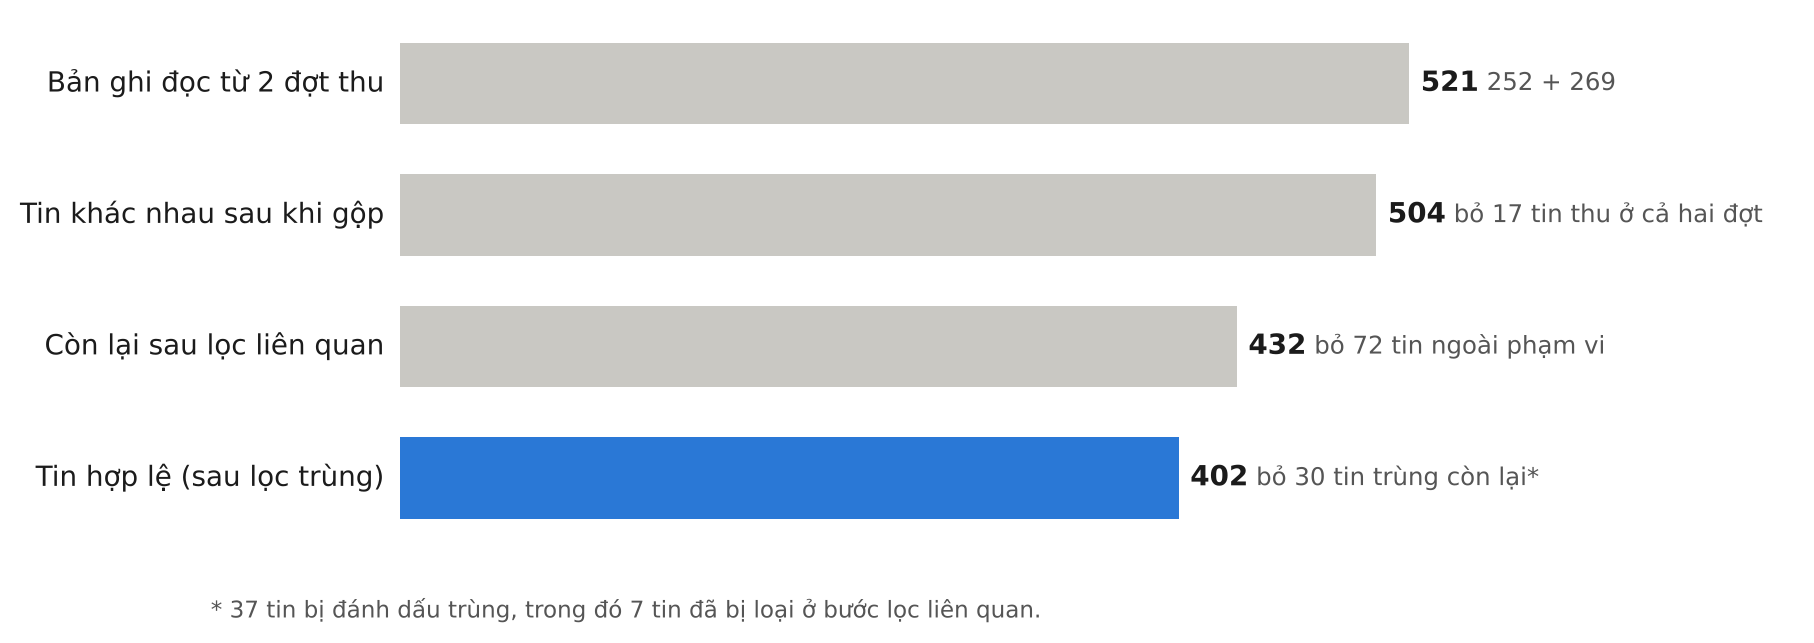
\includegraphics[width=0.95\textwidth]{image/funnel.png}}{\fbox{funnel.png}}
\caption{Từ 521 bản ghi của hai đợt thu đến 402 tin hợp lệ}
\label{fig:funnel}
\end{figure}

Trong 504 tin khác nhau, 72 tin bị loại vì ngoài phạm vi (đều là \code{NOT\_DATA\_AI\_ROLE}) và 37 tin bị đánh dấu trùng gần, trong đó 7 tin vừa trùng vừa ngoài phạm vi. Số tin hợp lệ là $504 - 72 - 37 + 7 = 402$. Theo đợt: pilot có 209 hợp lệ, 38 ngoài phạm vi, 5 trùng; đợt 03/11 có 193 hợp lệ, 34 ngoài phạm vi, 25 trùng. Không có lỗi kỹ thuật (\code{SCRAPE\_ERROR}).

Trên bộ pilot 252 tin, các cờ chất lượng đếm được: thiếu kinh nghiệm 252, thiếu địa điểm 83, đã bỏ cấp bậc khỏi chức danh 74, cần rà soát tay 39, đã bỏ nhiễu tuyển dụng 24, địa điểm không nhận diện được 18, đã bỏ hậu tố công nghệ 13.

\subsection{Phân tích khám phá dữ liệu}
\label{sec:eda}

\dacoi{} Mã ở \code{src/analysis/eda.py} và notebook \code{notebooks/eda.ipynb}, chạy trên 504 tin thô và bảng sạch ngày 04/11/2026. Chỉ số tổng hợp ở Bảng~\ref{tab:eda}.

\begin{table}[htbp]
\centering
\caption{Số liệu tổng quan của bộ dữ liệu (sơ bộ, 04/11/2026)}
\label{tab:eda}
\renewcommand{\arraystretch}{1.15}
\begin{tabular}{l l}
\toprule
\textbf{Chỉ số} & \textbf{Giá trị} \\
\midrule
Tin khác nhau / tin hợp lệ & 504 / 402 \\
Ngày đăng & 11/08/2026 -- 03/11/2026 \\
Số công ty (tin hợp lệ) & 239; 166 công ty chỉ đăng 1 tin \\
Tỉ trọng 10 công ty đăng nhiều nhất & 18,2\% \\
Độ dài trung vị mô tả + yêu cầu & 2.567 ký tự \\
Ngôn ngữ (tin hợp lệ) & tiếng Anh 63\%, tiếng Việt 37\% \\
Số kỹ năng mỗi tin & trung bình 10,6, trung vị 8; vài tin trên 30 \\
Số chức danh chuẩn hoá khác nhau & 347 cho 402 tin \\
\bottomrule
\end{tabular}
\end{table}

\textbf{Dữ liệu thiếu.} Chức danh, công ty, mô tả, yêu cầu và ngày đăng đủ 100\%. Địa điểm không lấy được ở 29\% tin, kinh nghiệm ở 100\%. Kiểm tra lại cho thấy cả hai chủ yếu là \textbf{giới hạn của crawler}, không phải ITviec không có thông tin: crawler chỉ đọc một trường địa điểm trong JSON-LD (130 tin ở đó ghi ``Not Available'') và tìm kinh nghiệm ở các vị trí đoán trước chưa từng khớp trang thật. Phải sửa crawler trước đợt 15/11.

\textbf{Ngôn ngữ.} 37\% tin viết tiếng Việt (ước lượng bằng tỉ lệ chữ có dấu tiếng Việt, ngưỡng 5\%). Taxonomy hiện chỉ có một tên gọi tiếng Việt, nên các tin này bị bỏ sót kỹ năng nhiều hơn (mục~\ref{sec:res-parser}).

\textbf{Thời gian.} Mỗi đợt thu chủ yếu bắt tin đăng trong sáu tuần trước đó; hai đợt cách nhau 34 ngày gần như không chồng nhau (Hình~\ref{fig:dates}). Dữ liệu là chuỗi ``ảnh chụp'' theo thời gian, không phải mọi tin đã từng đăng.

\begin{figure}[htbp]
\centering
\IfFileExists{image/eda_posted_dates.png}{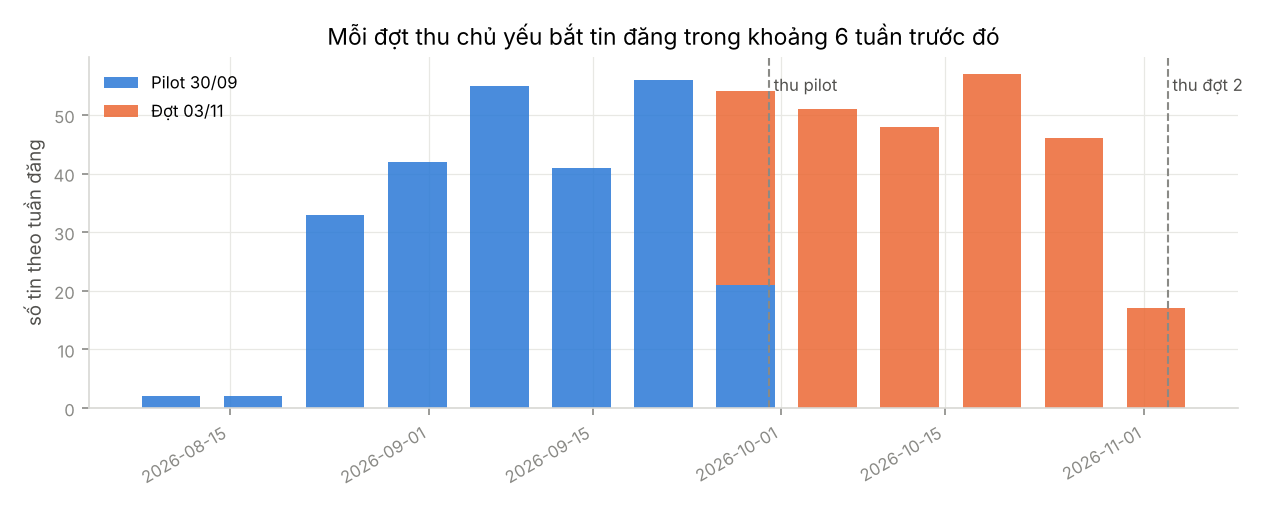
\includegraphics[width=0.85\textwidth]{image/eda_posted_dates.png}}{\fbox{eda\_posted\_dates.png}}
\caption{Số tin theo tuần đăng, tô màu theo đợt thu}
\label{fig:dates}
\end{figure}

\textbf{Công ty.} Không công ty nào chi phối: 239 công ty, 10 công ty lớn nhất chỉ chiếm 18\%. Ngân hàng tuyển nhiều (MB Bank 17 tin, cùng VietinBank, PVcomBank, HDBank).

\textbf{Nhóm kỹ năng.} Hình~\ref{fig:groups} cho tỉ lệ tin có ít nhất một kỹ năng của mỗi nhóm trong 15 nhóm. Ngôn ngữ lập trình và truy vấn đứng đầu (67\%); Cloud (43\%) và DevOps/MLOps (42\%) xấp xỉ các nhóm lõi Data/AI như AI tạo sinh (40\%) và học máy (36\%). Kiểm tra riêng 217 tin có chức danh Data/AI cho thấy Cloud (53\%) và DevOps (50\%) vẫn đứng đầu: đây chủ yếu là \textbf{đặc điểm thật của thị trường} (kỹ sư dữ liệu làm trên AWS/GCP, kỹ sư ứng dụng LLM cần CI/CD và Docker), không phải dấu hiệu lỗi. Một phần nhỏ do từ ``cloud'' trơn được nhận là Cloud Computing (43 trên 173 tin chỉ có Cloud nhờ từ này) và do tin IT chung lọt bộ lọc. Lưu ý: nhóm nhiều kỹ năng dễ ``trúng'' hơn (Cloud có 20 kỹ năng, NLP chỉ 3), và một tin có thể thuộc nhiều nhóm.

\begin{figure}[htbp]
\centering
\IfFileExists{image/eda_skill_groups.png}{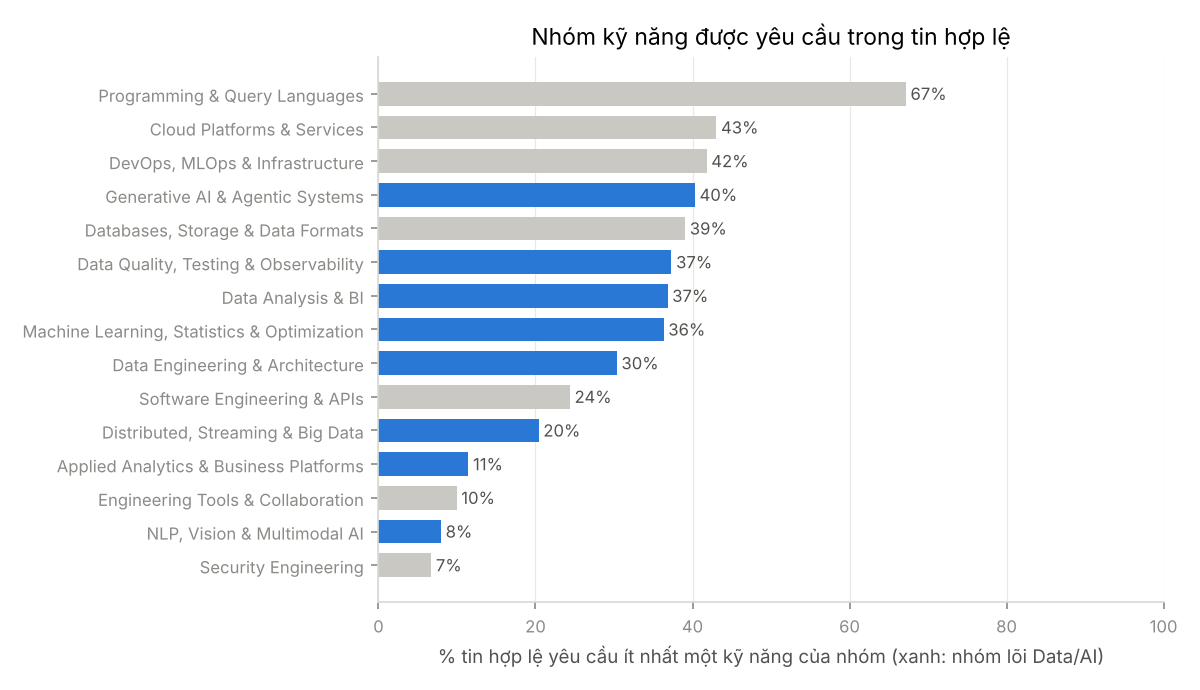
\includegraphics[width=0.9\textwidth]{image/eda_skill_groups.png}}{\fbox{eda\_skill\_groups.png}}
\caption{Tỉ lệ tin hợp lệ có ít nhất một kỹ năng của mỗi nhóm}
\label{fig:groups}
\end{figure}

\textbf{Kiểm tra bộ lọc liên quan.} Nhóm chạy bộ trích xuất trên \textbf{mọi} tin, kể cả tin bị loại, rồi tính với mỗi tin \textit{tỉ lệ kỹ năng lõi Data/AI}: số kỹ năng thuộc tám nhóm lõi (phân tích và BI, kỹ nghệ dữ liệu, học máy và thống kê, AI tạo sinh, NLP và thị giác, dữ liệu lớn, chất lượng dữ liệu, phân tích ứng dụng) chia cho tổng số kỹ năng của tin. Python và SQL không tính là lõi vì dùng chung với kỹ sư phần mềm nên không phân biệt được tin Data/AI. Tin được chia theo chức danh bằng từ khoá thô, chỉ để mô tả.

\begin{table}[htbp]
\centering
\caption{Tỉ lệ kỹ năng lõi Data/AI theo nhóm tin (sơ bộ)}
\label{tab:filter}
\renewcommand{\arraystretch}{1.15}
\begin{tabular}{l r r r}
\toprule
\textbf{Nhóm tin} & \textbf{Số tin} & \textbf{Kỹ năng TB} & \textbf{Tỉ lệ lõi (trung vị)} \\
\midrule
Giữ, chức danh Data/AI & 217 & 14,5 & 57\% \\
Bị loại vì ngoài phạm vi & 72 & 10,7 & 40\% \\
Giữ, chức danh IT chung & 117 & 7,6 & \textbf{29\%} \\
Giữ, Business Analyst & 68 & 3,1 & 25\% \\
\bottomrule
\end{tabular}
\end{table}

117 tin IT chung đang được giữ có tỉ lệ kỹ năng lõi \textbf{thấp hơn} cả các tin đã bị loại. Bộ lọc sai theo cả hai chiều: trong số tin bị loại có ``AI Software Engineer'' và ``Principal Software Engineer (LLM Agents)'', bị loại vì chứa ``software engineer'' dù có thể thuộc phạm vi AI. Trong 68 tin Business Analyst, 28 tin không khớp từ khoá nào và được giữ theo mặc định, 24 tin khớp đúng một từ khoá (thường là ``sql''); 6 tin khớp ``học máy'' do nằm trong cụm ``khoa học máy tính''. Tin BA trung bình chỉ có 3 kỹ năng kỹ thuật vì mô tả công việc chủ yếu bằng nghiệp vụ.

\begin{figure}[htbp]
\centering
\IfFileExists{image/eda_filter_check.png}{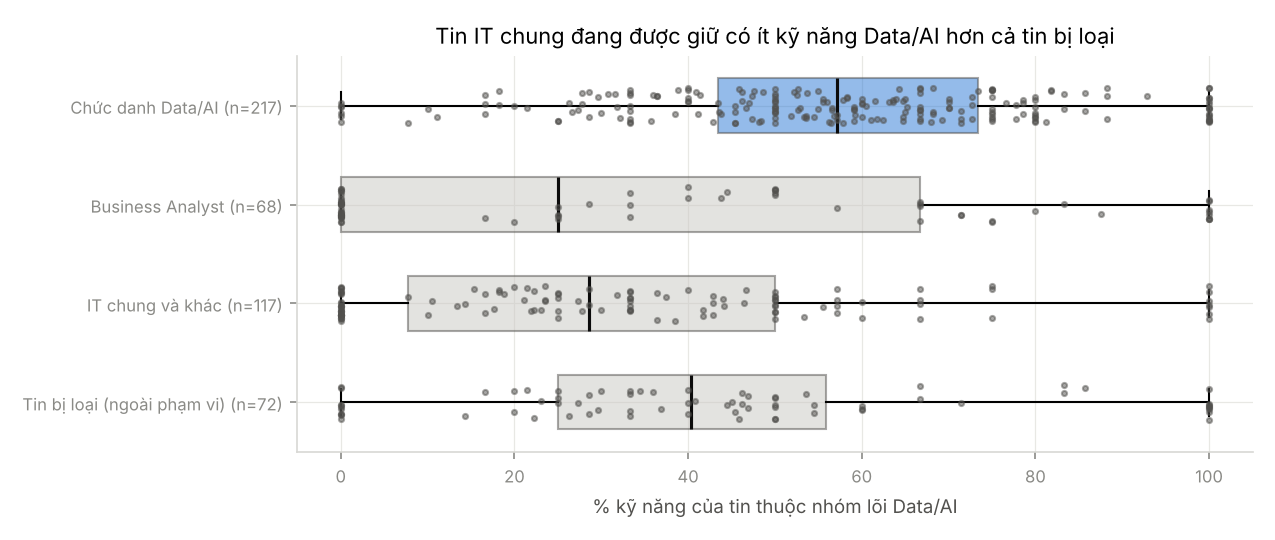
\includegraphics[width=0.9\textwidth]{image/eda_filter_check.png}}{\fbox{eda\_filter\_check.png}}
\caption{Tỉ lệ kỹ năng lõi Data/AI của từng tin, theo nhóm}
\label{fig:filter}
\end{figure}

\textbf{Hệ quả.} Bộ lọc cần siết trước ngày chốt. Hướng xử lý \dachot{} (07/11): giữ tin BA trong dữ liệu nhưng gán đúng vai trò khi gán nhãn (BA làm dữ liệu thuộc DA, BA nghiệp vụ là lớp riêng), và dùng nhãn \code{OTHER} của Nhiệm vụ 1 để học cách nhận ra tin không phải Data/AI thay cho quy tắc ``một từ khoá''.

\newpage
% =====================================================================
\section{Phương pháp}
% =====================================================================
\subsection{Kiến trúc đường ống và hợp đồng giữa các khâu}
\label{sec:pipeline}

\begin{figure}[htbp]
\centering
\begin{tikzpicture}[
  box/.style={draw, rounded corners=2pt, minimum height=1.3cm, text width=2.35cm, align=center, font=\small},
  arr/.style={-{Stealth[length=2.2mm]}, thick}]
\node[box] (a) {\textbf{Crawl}\\ITviec, dữ liệu thô JSONL};
\node[box, right=0.4cm of a] (b) {\textbf{Clean}\\22 trường, cờ trùng và liên quan};
\node[box, right=0.4cm of b] (c) {\textbf{Extract}\\taxonomy, danh sách và ma trận};
\node[box, right=0.4cm of c] (d) {\textbf{Analysis}\\8 kiểm tra, EDA, RQ2--RQ4};
\node[box, right=0.4cm of d] (e) {\textbf{App}\\Skill Navigator (kế hoạch)};
\node[box, below=0.6cm of b] (r1) {\textbf{RQ1}\\thống kê chức danh};
\node[box, below=0.6cm of c] (g) {\textbf{Đánh giá}\\gold, P/R/F1};
\draw[arr] (a) -- (b); \draw[arr] (b) -- (c); \draw[arr] (c) -- (d); \draw[arr] (d) -- (e);
\draw[arr] (b) -- (r1); \draw[arr, dashed] (g) -- (c);
\end{tikzpicture}
\caption{Kiến trúc đường ống. Nét đứt: bộ đánh giá chấm bộ trích xuất.}
\label{fig:pipeline}
\end{figure}

\dacoi{} Khung tích hợp ở \code{src/pipeline/} (Dương phụ trách) đọc cấu hình \code{config/pipeline.json}, gọi module của từng thành viên, kiểm tra hợp đồng dữ liệu trước và sau mỗi khâu, rồi mới chuyển bước. Logic làm sạch, trích xuất và phân tích nằm trong module của người phụ trách; khung không viết lại chúng.

\begin{table}[htbp]
\centering
\caption{Phân công theo khâu (quyết định 03/10 và 03/11/2026)}
\label{tab:owners}
\renewcommand{\arraystretch}{1.15}
\begin{tabularx}{\textwidth}{>{\raggedright\arraybackslash}p{4.6cm} l X}
\toprule
\textbf{Khâu} & \textbf{Người phụ trách} & \textbf{Entry point} \\
\midrule
Thu thập & Đạt & \code{src.crawler.main} \\
Làm sạch, chuẩn hoá chức danh, RQ1 & Đức & \code{src.cleaner.pipeline}, \code{src.cleaner.rq1:run} \\
Taxonomy, trích xuất, gold, P/R/F1 & Cường & \code{src.parser.features:run} \\
RQ2--RQ4 & Triều & \code{src.analysis.report:run} \\
Phạm vi, lược đồ, điều phối, nghiệm thu & Dương & \code{src.pipeline} \\
\bottomrule
\end{tabularx}
\end{table}

\textbf{Cách chạy.} \code{python -m src.pipeline --config <tệp cấu hình> --stage all} chạy \code{clean}, \code{rq1}, \code{extract}, \code{analysis} theo thứ tự và dừng ở lỗi đầu tiên; có thể chạy riêng từng bước. Sau khi đã có bảng sạch, \code{extract} không cần dữ liệu thô, và \code{analysis} chỉ cần bảng sạch, hai bảng đặc trưng và taxonomy, nên sửa bộ trích xuất thì chỉ chạy lại hai bước cuối. Mã thoát 0 khi hợp lệ, 1 khi lỗi cấu hình, thiếu module, thiếu tệp hoặc sai hợp đồng. Seed cố định nên chạy lại ra đúng số cũ.

\textbf{Hợp đồng.} Mỗi module là một hàm \code{run(context)}; \code{context.paths} chứa đường dẫn các tệp, \code{context.options} chứa cấu hình của bước, cả hai chỉ đọc. Khung kiểm tra: đủ 22 trường, đúng kiểu, \code{job\_id} duy nhất, cờ là boolean thật, có lý do loại khi bị loại, trường gốc không bị sửa, tập \code{job\_id} giữ nguyên từ thô sang sạch; bảng kỹ năng và ma trận đúng tập tin hợp lệ, cột ma trận thuộc taxonomy, danh sách và ma trận khớp từng ô. Module phân tích trả trạng thái mỗi RQ: \code{completed} phải có tệp không rỗng, \code{skipped} phải có lý do. Đầu ra chỉ được thay sau khi toàn bộ hợp đồng của bước đạt.

\textbf{Báo cáo lần chạy.} Mỗi lần chạy ghi thời gian, hash cấu hình và từng tệp đầu vào, số bản ghi, trạng thái từng bước và từng RQ. Vì tin trùng và tin ngoài phạm vi có thể giao nhau: $\text{bản ghi sạch} = \text{hợp lệ} + \text{trùng} + \text{ngoài phạm vi} - \text{giao}$. Cờ \code{research\_acceptance = true} chỉ khi chạy chế độ nghiên cứu, toàn chuỗi thành công và cả bốn RQ \code{completed}; trưởng nhóm vẫn phải nghiệm thu chất lượng. Khung có 49 kiểm thử tích hợp dùng module giả lập.

\subsection{Taxonomy kỹ năng}
\label{sec:taxonomy}

\textbf{Định nghĩa.} Một \textbf{kỹ năng kỹ thuật} là năng lực học được, phương pháp, công cụ, ngôn ngữ, thư viện, nền tảng, hệ thống dữ liệu, kỹ thuật phân tích hoặc miền kỹ thuật được nêu rõ trong tin như một phần của công việc Data/AI. Phương pháp như Machine Learning, ETL, A/B Testing, RAG, MLOps cũng là kỹ năng. Kỹ năng mềm, phẩm chất cá nhân, ngoại ngữ, bằng cấp, số năm kinh nghiệm, cấp bậc, nhãn nghề (``Data Engineer'') và thuật ngữ quá rộng (``AI'', ``Data'') không phải kỹ năng.

\textbf{Cấu trúc.} \dacoi{} \code{taxonomy/skills\_taxonomy.csv} có các cột \code{skill\_id}, \code{canonical\_name}, \code{abbreviation}, \code{aliases}, \code{skill\_group}, \code{observed\_count}; gồm \textbf{246 kỹ năng} chia 15 nhóm, 34 kỹ năng có viết tắt và tổng 82 tên gọi khác. Cường xây taxonomy \textbf{từ dữ liệu}: đếm kỹ năng trong 45 tin mẫu ITviec (\code{data/sample/sample\_jobs.jsonl}) và bỏ kỹ năng không xuất hiện. \code{observed\_count} là số tin trong mẫu có nhắc kỹ năng ít nhất một lần: 103 kỹ năng xuất hiện đúng một lần, 150 kỹ năng tối đa hai lần. Số này chỉ kiểm tra taxonomy, không phải nhu cầu thị trường. \code{skill\_group} chỉ dùng để quản lý từ vựng, \textbf{không phải danh mục nghề} và không được đưa vào phân cụm.

\textbf{Quản lý thay đổi.} \dachot{} Không tái sử dụng \code{skill\_id} cho khái niệm khác; tên gọi khác được bổ sung qua taxonomy, không viết thêm danh sách trong mã; đổi tên chuẩn phải có lý do và nhật ký. \textbf{Taxonomy và bộ trích xuất bị khoá ngày 23/11/2026}; trước đó chỉ được bổ sung tên gọi khác dựa trên lỗi ở nửa \textit{tune} của gold (mục~\ref{sec:gold}). \code{python scripts/recount\_taxonomy.py --check} kiểm tra lại số đếm.

\subsection{Bộ trích xuất kỹ năng}
\label{sec:parser}

\dacoi{} \code{src/parser/skill\_extractor.py} là thuật toán duy nhất; \code{recount\_taxonomy.py} và đường ống dùng chung nó.

\begin{algorithm}[htbp]
\caption{Trích kỹ năng từ văn bản một tin}
\label{alg:parser}
\begin{algorithmic}[1]
\Require văn bản $x$ (\code{job\_text}), taxonomy $T$
\Ensure danh sách tên chuẩn, không trùng, theo thứ tự taxonomy
\State chuẩn hoá $x$ theo NFKC
\For{mỗi kỹ năng $s \in T$ và mỗi dạng viết $v$ của $s$ (tên chuẩn, viết tắt, tên gọi khác)}
  \State tìm $v$ trong $x$ với ranh giới từ; C, R, Go phân biệt chữ hoa
  \State bỏ C nằm trong C++/C\#, R nằm trong R\&D
  \State với ``CV'': chỉ nhận khi văn bản có ngữ cảnh thị giác máy tính
\EndFor
\State các đoạn khớp chồng nhau: giữ đoạn dài hơn (``SQL Server'' thắng ``SQL'')
\State khử trùng theo \code{skill\_id}; \Return tên chuẩn
\end{algorithmic}
\end{algorithm}

Ví dụ: ``Experience in Python, SQL Server and Power BI.'' cho \{Microsoft SQL Server, Power BI, Python\}; ``Send us your CV.'' cho danh sách rỗng.

\textbf{Đầu ra.} Lệnh \code{python -m src.parser extract} chỉ xử lý tin \code{relevance\_flag = true AND duplicate\_flag = false}, xuất \code{job\_skills.parquet} (mỗi tin một dòng, kể cả tin không có kỹ năng) và \code{job\_skill\_matrix.parquet} (cột \code{skill\_id}, giá trị 0/1). Khi phân tích, kỹ năng xuất hiện ở dưới 3 tin bị bỏ khỏi ma trận.

\textbf{Giới hạn đã biết.} Ba kiểm thử \code{xfail(strict=True)} giữ lại các giới hạn chưa sửa: phủ định (``Python is not required'' vẫn bắt Python), ``Go'' ở đầu câu, và ``CV'' (hồ sơ) trong tin có ngữ cảnh thị giác. Ngoài ra: taxonomy gần như không có tên tiếng Việt; thiếu nhiều tên gọi khác (``REST API'' không được nhận là API Design); bộ trích xuất đọc cả phần giới thiệu công ty. Công cụ ngoài taxonomy (OpenCV, Hugging Face) chỉ ghi ở \code{taxonomy/taxonomy\_gaps.csv}.

\subsection{Bộ đáp án kỹ năng (gold) và quy trình gán nhãn}
\label{sec:gold}

\textbf{Chọn mẫu.} \dacoi{} 50 tin thật từ đợt pilot (\code{data/evaluation/gold\_jobs.draft.jsonl}). Loại mọi tin trùng \code{job\_id}, \code{source\_url} hoặc \code{source\_job\_id} với 45 tin dùng xây taxonomy, và loại cặp có văn bản giống nhau từ 0,5 trở lên (Jaccard trên cụm 5 từ). Lọc chức danh có Data, AI, Machine Learning hoặc Business Intelligence, rồi lấy \textbf{50 tin ngắn nhất} cho dễ gán. Đây là thiên lệch đã biết: độ dài trung vị của gold khoảng 2.000 ký tự, của toàn bộ dữ liệu 2.567.

\textbf{Ba lớp gán nhãn.}
\begin{enumerate}[noitemsep, topsep=2pt, leftmargin=2.5em]
\item \textit{Nhãn nháp.} Trợ lý AI (Codex) đọc từng tin và gán 634 nhãn, mỗi nhãn kèm đoạn bằng chứng (vị trí ký tự trên trường \code{text}). Nhãn được gán \textbf{trước} khi chạy bộ trích xuất trên tập này nên không chép từ kết quả bộ trích xuất. Mọi bản ghi có \code{human\_reviewed = false}.
\item \textit{Rà soát lượt hai.} Một trợ lý AI khác (Claude) đọc lại và đưa 99 góp ý trong \code{review\_pass2.jsonl}: 24 nhãn đáng ngờ (12 sửa bằng chứng, 1 đổi kỹ năng, 11 cần xem) và 75 kỹ năng có thể bị sót (25 mức cao, 50 cần xem). Góp ý không sửa gold.
\item \textit{Người duyệt.} Dương và Cường duyệt từng nhãn và góp ý trên trang \code{tools/gold\_review/index.html} chạy offline, theo hướng dẫn ở Phụ lục~\ref{app:skill-guideline}. Chỉ sau bước này bản ghi mới có \code{human\_reviewed = true}. \textbf{Không sửa nhãn để khớp bộ trích xuất.}
\end{enumerate}

\textbf{Quy ước chung.} Quyết định của người được áp dụng cho mọi tin. Ví dụ ngày 05/11/2026, Cường quyết định tin nhắc tới xây dựng, tích hợp hay làm việc với API đều gán API Design; 12 góp ý loại này được đánh dấu \code{auto = add}, trang duyệt hiện ``đã thêm theo quy ước'' và script gộp luôn thêm chúng.

\textbf{Kiểm tra độ đồng ý.} \dacoi{} 18 tin cố định (18 \code{job\_id} đầu khi sắp theo \code{sha256("kappa-v1:" + job\_id)}). Với các tin này, trang duyệt \textbf{ẩn nhãn nháp} cho đến khi người duyệt gán độc lập xong. \code{scripts/merge\_gold\_reviews.py} gộp các tệp duyệt thành \code{gold\_jobs.reviewed.jsonl}, tính Cohen's kappa trên mọi cặp (tin, kỹ năng) của 18 tin $\times$ 246 kỹ năng cùng đồng thuận dương, và ghi bất đồng vào \code{review\_conflicts.csv}.

\textbf{Chia tune/holdout.} \dachot{} (F.9) Hàm \code{gold\_split()} tính \code{sha256("gold-split-v1:" + job\_id)}, lấy 8 ký tự hex đầu đổi thành số: chẵn vào \textit{holdout}, lẻ vào \textit{tune}. Ví dụ \code{6d8a728e0459f4b4} cho \code{7e57a230} (chẵn, holdout); \code{61f8d549b3cc6002} cho \code{70a79ff3} (lẻ, tune). Kết quả: 27 tin tune, 23 tin holdout. Chỉ được xem lỗi trên nửa tune; không mở \code{errors.jsonl} hay \code{predictions.jsonl} của nửa holdout trước ngày khoá 23/11/2026; điểm chính thức báo cáo trên holdout. Không ai chọn tay tin vào nhóm nào, và thêm tin mới không làm tin cũ đổi nhóm.

\subsection{Phân tích RQ1--RQ4}
\label{sec:analysis}

Các ngưỡng và phương pháp được viết ra \textbf{trước} khi có dữ liệu đầy đủ, để không chọn sau cho đẹp số. Mọi RQ chỉ dùng tin hợp lệ. Mã ở \code{src/analysis/} (Triều), ngưỡng ở \code{src/analysis/config.py}.

\textbf{RQ1} \dacoi{} (\code{src/cleaner/rq1.py}). Số tin hợp lệ; số chức danh thô (trim + chữ thường) và chuẩn hoá khác nhau; tỉ lệ nén (chuẩn hoá $\div$ thô); độ tập trung (tỉ trọng top 1, 5, 10; HHI); entropy Shannon; tỉ lệ chức danh hiếm ($\le 2$ tin) và \textbf{các công ty đứng sau chức danh hiếm}, để phân biệt ``vài công ty tự đặt tên'' với ``thị trường phân mảnh''.

\textbf{RQ2} \dacoi{} (\code{rq2.py}). Tần suất kỹ năng; số kỹ năng mỗi tin (trung bình, trung vị, p10, p90) để kiểm tra sức khoẻ bộ trích xuất; đồng xuất hiện và ba thước đo cặp: lift, NPMI, Jaccard, vì mỗi thước đo có một điểm yếu (lift phóng đại cặp hiếm, Jaccard thiên về cặp phổ biến). Cộng đồng kỹ năng tìm bằng thuật toán trên mạng đồng xuất hiện, không gom tay.

\textbf{RQ3} \dacoi{} (\code{rq3.py}). Kiểm tra 1: độ phân tán của mỗi chức danh so với 1.000 lần bốc ngẫu nhiên cùng cỡ (mục~\ref{sec:jaccard}). Kiểm tra 2: hồ sơ kỹ năng của mỗi chức danh (vector tỉ lệ), cosine giữa các hồ sơ; cặp vượt 0,70 / 0,80 / 0,90 được đánh dấu là có thể cùng một việc \dexuat{} (ba ngưỡng chờ trưởng nhóm duyệt).

\textbf{RQ4} \dacoi{} (\code{rq4.py}). Phân cụm trên không gian kỹ năng, \textbf{chức danh bị giấu}. Quét $k$ từ 2 đến 15; với mỗi $k$ tính silhouette, Davies--Bouldin và độ ổn định (100 lần, mẫu 80\%, K-Means \code{n\_init = 10}, seed 42). Đối chứng bằng phân cụm phân cấp (Jaccard, liên kết trung bình) cùng $k$, so bằng ARI. PCA để vẽ. Cụm $\times$ chức danh và ARI/NMI giữa cụm và chức danh chỉ tính \textbf{sau} khi đã ghi nhãn cụm.

\textbf{Luật chọn $k$} \dachot{} (03/11/2026, F.11): giữ các $k$ có độ ổn định cách mức cao nhất không quá 0,02; trong đó giữ các $k$ có silhouette cách mức cao nhất không quá 0,02; chọn $k$ nhỏ nhất còn lại. Độ ổn định xếp trước vì một cụm trông tách biệt mà biến mất khi lấy mẫu lại chỉ là đặc thù của mẫu. Thứ tự này được kiểm trên dữ liệu giả có bốn nhóm cài sẵn: xét silhouette trước khi lấy $k$ nhỏ chọn đúng $k = 4$ (ARI 0,99), nếu không sẽ chọn $k = 3$ (ARI 0,71). Toàn bộ kết quả quét được công bố.

\textbf{Đề xuất đổi khoảng cách} \dexuat{}. K-Means hiện dùng khoảng cách Euclid trên ma trận 0/1 và chia tin theo độ dài (mục~\ref{sec:res-rq4}). Đề xuất chuẩn hoá mỗi hàng về độ dài 1 trước khi chạy (tương đương cosine) và thêm mốc dữ liệu xáo trộn (mục~\ref{sec:clustering}). Lý do là nguyên tắc phương pháp, không phải vì kết quả đẹp hơn; thay đổi phải được chốt trước bản chạy chính thức.

\begin{table}[htbp]
\centering
\caption{Các ngưỡng định lượng (chốt trước khi xem dữ liệu thật, giữ nguyên 03/11/2026)}
\label{tab:thresholds}
\renewcommand{\arraystretch}{1.15}
\begin{tabularx}{\textwidth}{l c X}
\toprule
\textbf{Ngưỡng} & \textbf{Giá trị} & \textbf{Lý do} \\
\midrule
Tin mỗi chức danh (RQ3) & $\ge 5$ & 5 tin tạo 10 cặp; ít hơn thì trung bình không phân biệt được với ngẫu nhiên \\
Số chức danh đạt ngưỡng trên (RQ3) & $\ge 3$ & Dưới mức này không báo cáo RQ3 \\
Tin mỗi kỹ năng & $\ge 3$ & Dưới 3 tin chỉ là nhiễu \\
Đồng xuất hiện mỗi cặp & $\ge 5$ & Lift biến động mạnh dưới ngưỡng này \\
Kỹ năng mỗi tin khi đo tương đồng & $\ge 2$ & Một kỹ năng thì không có gì để so \\
Số tin tối thiểu để phân cụm & $\ge 300$ & Dưới mức này cụm chỉ là ngẫu nhiên \\
\bottomrule
\end{tabularx}
\end{table}

\textbf{Mẫu nhỏ.} Với tập 30--50 tin, chỉ được chạy thử đường ống (đếm tin, đếm chức danh, tần suất kỹ năng, kiểm tra chất lượng); các phép đo cần phân phối thật (độ tập trung, cặp kỹ năng, RQ3, RQ4) phải bỏ hẳn, không công bố kèm cảnh báo, vì con số kèm cảnh báo vẫn bị trích dẫn. Nếu đến 23/11/2026 vẫn dưới 300 tin hợp lệ thì không hạ ngưỡng: RQ4 chỉ được trình bày như phương pháp kiểm chứng trên dữ liệu giả (F.13).

\textbf{Tám bước kiểm tra chất lượng} \dacoi{} (\code{src/analysis/quality.py}). Chạy trước mọi phân tích; một bước không đạt thì RQ2--RQ4 trả \code{skipped} kèm lý do (trừ khi chạy với \code{--ignore-quality} để chẩn đoán).

\begin{table}[htbp]
\centering
\caption{Tám bước kiểm tra chất lượng trước phân tích}
\label{tab:qc}
\renewcommand{\arraystretch}{1.12}
\begin{tabularx}{\textwidth}{c X c X}
\toprule
\textbf{Mã} & \textbf{Kiểm tra} & \textbf{Ngưỡng} & \textbf{Lỗi bắt được} \\
\midrule
QC1 & \code{job\_id} khớp 1--1 giữa bảng sạch và bảng kỹ năng & 0 lệch & Hai khâu chạy trên hai bộ dữ liệu khác nhau \\
QC2 & \code{extracted\_skills} không null & 0 & Bộ trích xuất chưa chạy hết \\
QC3 & Số kỹ năng trung bình mỗi tin & $\ge 3$ & Trích xuất yếu \\
QC4 & Tỉ lệ tin không có kỹ năng & $\le 10\%$ & Taxonomy thiếu mảng lớn, crawler lấy sai văn bản \\
QC5 & Tỉ lệ tin của kỹ năng phổ biến nhất & $\le 90\%$ & Tên gọi quá rộng, bắt nhầm từ thông dụng \\
QC6 & Trùng còn sót & $\le 2\%$ & Khử trùng bỏ sót \\
QC7 & Độ dài trung vị mô tả + yêu cầu & $\ge 300$ ký tự & Crawler cắt mất nội dung \\
QC8 & Tin thiếu \code{normalized\_job\_title} & 0 & Tin rơi khỏi RQ1, RQ3, RQ4 \\
\bottomrule
\end{tabularx}
\end{table}

\subsection{Nhận diện vai trò: nhãn và phương pháp}
\label{sec:roles}

\textbf{Bảy vai trò} \dachot{} (07/11/2026): \code{DA} phân tích dữ liệu và BI; \code{DE} kỹ nghệ và quản trị dữ liệu; \code{DS} khoa học dữ liệu; \code{MLE} kỹ sư học máy, gồm MLOps; \code{AIE} kỹ sư ứng dụng AI/LLM; \code{BA} phân tích nghiệp vụ; \code{OTHER} không phải Data/AI. Câu hỏi quyết định khi gán: \textit{đầu ra chính của người này là gì?} Định nghĩa đầy đủ, cách phân xử các cặp dễ nhầm và ví dụ ở Phụ lục~\ref{app:role-guideline}. MLOps gộp vào MLE vì chỉ có 2 tin; BA làm SQL và dashboard xếp vào DA, BA nghiệp vụ là lớp riêng để ứng dụng cảnh báo được người dùng.

\textbf{Mẫu gán nhãn} \dacoi{} (\code{scripts/sample\_role\_labeling.py}, \code{data/labels/role\_sample.csv}). 300 tin gồm \textbf{toàn bộ 65 tin bị bộ lọc loại} (không tính tin trùng), để đánh giá lại bộ lọc, cộng 235 tin hợp lệ chọn theo hàm băm \code{sha256("role-sample-v1:" + job\_id)}. Chia lô theo \code{sha256("role-batch-v1:" + job\_id)}: lô K gồm 60 tin, hai người gán độc lập để đo kappa; năm lô B1--B5, mỗi lô 48 tin, mỗi người một lô. Khối lượng khoảng 1--2 phút mỗi tin.

\textbf{Công cụ} \dacoi{} \code{tools/role\_labeling/} dựng trang \code{index.html} chạy offline. Trang \textbf{ẩn chức danh và tên công ty} để người gán không bị tên dẫn dắt, có phím 1--7, vai trò phụ, ô ``phân vân'' và ghi chú; xuất tệp JSON chỉ chứa mã tin và nhãn. Vì nhúng văn bản tin, \code{index.html} không được commit (kho mã công khai). \code{scripts/merge\_role\_labels.py} gộp các tệp, tính kappa từng cặp người gán, liệt kê bất đồng vào \code{role\_conflicts.csv}; kết quả họp thống nhất ghi vào \code{role\_adjudicated.csv}.

\textbf{Các phương pháp cho Nhiệm vụ 1} \dexuat{}. Tập nhãn được chia train/test cố định bằng hàm băm; điểm chấm là macro-F1 trên tập test.
\begin{table}[htbp]
\centering
\caption{Các phương pháp nhận diện vai trò sẽ so sánh}
\label{tab:methods}
\renewcommand{\arraystretch}{1.15}
\begin{tabularx}{\textwidth}{>{\raggedright\arraybackslash}p{5.2cm} X}
\toprule
\textbf{Phương pháp} & \textbf{Trả lời câu hỏi} \\
\midrule
Đoán vai trò từ chức danh (luật từ khoá) & Mốc; độ sai chính là mức chức danh đánh lừa \\
Có giám sát trên kỹ năng (hồi quy logistic, rừng ngẫu nhiên) & Danh sách kỹ năng có đủ để nhận ra vai trò không \\
Có giám sát trên văn bản (TF-IDF; embedding đa ngôn ngữ) & Văn bản đầy đủ có tốt hơn danh sách kỹ năng không \\
Không giám sát: K-Means (cosine), phân cụm phân cấp & Tìm vai trò không cần nhãn; đối chiếu nhãn bằng ARI \\
Mô hình hỗn hợp: LDA, NMF trên ``túi kỹ năng'' & Một tin thuộc nhiều vai trò, hợp với vai trò lai \\
LLM zero-shot & Mốc hiện đại \\
\bottomrule
\end{tabularx}
\end{table}

\textbf{Nhiệm vụ 2} \dexuat{}: tần suất kỹ năng trong mỗi vai trò; vị trí kỹ năng trong tin (mục ``Requirements'' hay ``Nice to have''); cộng đồng kỹ năng (Louvain) trên mạng đồng xuất hiện; độ đặc trưng (lift của kỹ năng trong vai trò so với các vai trò khác). Chấm bằng độ ổn định khi lấy mẫu lại và mức đồng thuận giữa các cách.

\textbf{Nhiệm vụ 3} \dexuat{}: độ tương đồng giữa hồ sơ người dùng và tin, có trọng số theo kỹ năng cốt lõi; gợi ý kỹ năng tiếp theo bằng luật kết hợp hoặc phân rã ma trận. Chấm không cần người: che ngẫu nhiên vài kỹ năng của một tin và đo Recall@5 khi đoán lại, so với mốc ``gợi ý kỹ năng phổ biến nhất''. Chấm có người: 8--10 sinh viên đọc 5 tin có và không có ứng dụng, đoán vai trò và kỹ năng bắt buộc, so độ đúng.

\textbf{Kiểm chứng nhu cầu} \dexuat{}: khảo sát 30--50 sinh viên IT (từng hiểu sai chức danh chưa; phân biệt được AI Engineer, ML Engineer, Data Scientist không; có biết kỹ năng nào bắt buộc; quyết định học gì dựa vào đâu; công cụ như vậy có giúp không), để có bằng chứng bài toán có thật.

\subsection{Giao thức đánh giá}
\label{sec:protocol}

Đồ án không có đáp án sẵn như bài toán dự đoán, nên đánh giá có hai tầng.

\textbf{Tầng 1 -- công cụ đo.} Bộ trích xuất được chấm trên gold (mục~\ref{sec:gold}); bộ nhận diện vai trò được chấm trên nhãn vai trò (mục~\ref{sec:roles}). Cả hai có hai người gán độc lập một phần để đo kappa, chia phần chỉnh và phần niêm phong cố định bằng hàm băm. Điểm báo cáo kèm khoảng tin cậy bootstrap 95\% (bốc lại theo \textit{tin}, 5.000 lần) và tách theo ngôn ngữ \dexuat{}.

\textbf{Tầng 2 -- kết quả phân tích.} Với mỗi kết quả, hỏi: dữ liệu ngẫu nhiên có cho ra kết quả này không? RQ2: tỉ lệ kèm khoảng tin cậy (ví dụ SQL 162/402 = 40,3\%, khoảng 35,5--45,1\%, nên không kết luận ``SQL hơn Python 39\%''); cặp chỉ xếp hạng khi cùng xuất hiện $\ge 5$ lần. RQ3: so với 1.000 lần bốc ngẫu nhiên. RQ4: độ ổn định, mốc dữ liệu xáo trộn, hai thuật toán đồng ý, chức danh chỉ đưa vào sau. Tất cả sau tám bước kiểm tra chất lượng.

\begin{table}[htbp]
\centering
\caption{Tiêu chí chấp nhận \dexuat{} (chờ giảng viên duyệt)}
\label{tab:acceptance}
\renewcommand{\arraystretch}{1.15}
\begin{tabularx}{\textwidth}{l X X}
\toprule
\textbf{Đối tượng} & \textbf{Tiêu chí} & \textbf{Nếu không đạt} \\
\midrule
Gold, nhãn vai trò & $\kappa \ge 0{,}6$ giữa hai người gán (mức ``đáng kể'') & Sửa hướng dẫn ở chỗ hai người hiểu khác, gán lại phần liên quan \\
Bộ trích xuất & Báo cáo P/R/F1 trên holdout kèm khoảng tin cậy và tách theo ngôn ngữ; không đặt mốc đỗ cứng & Ghi rõ hậu quả, ví dụ recall thấp thì tỉ lệ kỹ năng ở RQ2 thấp hơn thực tế \\
RQ2 & So hai tỉ lệ chỉ khi khoảng tin cậy không chồng nhau & Báo cáo là ``tương đương'' \\
RQ3 & Nhất quán khi độ phân tán $<$ phân vị 5\% của mốc ngẫu nhiên; cần $\ge 3$ chức danh có $\ge 5$ tin & Không báo cáo RQ3, ghi lý do \\
RQ4 & Chỉ trình bày nhóm nghề khi ổn định hơn và tách rõ hơn dữ liệu xáo trộn & Kết luận ``dữ liệu không cho thấy nhóm nghề rõ ràng'' \\
\bottomrule
\end{tabularx}
\end{table}

Ba luật chung: chốt cách chấm trước, chấm sau; không sửa nhãn để khớp bộ trích xuất; không mở phần niêm phong trước ngày khoá. Sau 23/11 nếu phát hiện lỗi bộ trích xuất thì ghi vào hạn chế; nếu buộc phải sửa thì báo cáo cả điểm trước và sau, ghi rõ holdout đã bị xem.

\newpage
% =====================================================================
\section{Kết quả thực nghiệm (sơ bộ)}
% =====================================================================
Mọi số liệu trong mục này là \textbf{sơ bộ}: dữ liệu chưa chốt, gold chưa được người duyệt xong, bộ lọc liên quan chưa siết. Số chính thức sẽ thay sau ngày 23/11/2026.

\subsection{Bộ trích xuất kỹ năng}
\label{sec:res-parser}

Chạy ngày 11/10/2026 trên gold nháp 50 tin, thuật toán và từ vựng cố định trong lần đánh giá.

\begin{table}[htbp]
\centering
\caption{Bộ trích xuất so với gold nháp (micro, theo cặp tin--kỹ năng)}
\label{tab:parser}
\renewcommand{\arraystretch}{1.15}
\begin{tabular}{l r}
\toprule
\textbf{Chỉ số} & \textbf{Giá trị} \\
\midrule
TP / FP / FN & 541 / 21 / 93 \\
Precision & 96,26\% \\
Recall & 85,33\% \\
F1 & 90,47\% \\
Tin có ít nhất một FP hoặc FN & 43 / 50 \\
\bottomrule
\end{tabular}
\end{table}

Ba biến thể của đáp án cho thấy điểm nhạy với chất lượng gold:
\begin{itemize}[noitemsep, topsep=2pt, leftmargin=2.5em]
\item Nhận mọi góp ý mức cao của lượt rà soát hai (gold 659 nhãn): P 96,1\%, R 81,9\%, F1 88,5\%. Phần lớn nhãn bị gold nháp sót cũng là chỗ bộ trích xuất sót, nên gold nháp làm recall trông cao hơn thực tế.
\item Chỉ thêm 12 nhãn API Design theo quy ước 05/11: P 96,3\%, R 83,7\%, F1 89,6\%; bộ trích xuất sót cả 12 vì taxonomy chỉ có tên gọi ``API architecture''.
\item Khoảng tin cậy bootstrap 95\% (bốc lại 50 tin, 5.000 lần) với biến thể trên: P 94,7--97,7\%; R 80,1--86,9\%; F1 87,2--91,7\%.
\end{itemize}

\textbf{Theo ngôn ngữ.} Tin tiếng Anh (33 tin): P 95,5\%, R 87,3\%. Tin tiếng Việt (17 tin): P 97,8\%, R \textbf{81,6\%}. Tên công nghệ trong tin tiếng Việt vẫn thường viết bằng tiếng Anh nên phần lớn vẫn bắt được; các khái niệm viết bằng tiếng Việt (``học máy'', ``bảo mật dữ liệu'', ``triển khai mô hình'') thì bị sót.

\begin{table}[htbp]
\centering
\caption{Các nhóm lỗi quan sát được}
\label{tab:parser-errors}
\renewcommand{\arraystretch}{1.15}
\begin{tabularx}{\textwidth}{>{\raggedright\arraybackslash}p{4.6cm} X}
\toprule
\textbf{Nhóm lỗi} & \textbf{Ví dụ} \\
\midrule
Thiếu tên gọi khác, số ít/nhiều & ``Database'' không khớp Databases; Oracle, MS SQL, Big Query, K8S; ``REST APIs'' \\
Thiếu tên tiếng Việt & ``bảo mật dữ liệu'', ``học máy'', ``triển khai mô hình'' \\
Trùng từ thông dụng & React khớp ReAct; ``fine-tuning'' cơ sở dữ liệu khớp Fine-Tuning của ML \\
Đọc cả vùng không phải yêu cầu & ngành học ``Statistics''; CI/CD ở phần giới thiệu công ty \\
Ranh giới khái niệm & Optimization, Reporting, Computer Vision từ ``facial recognition'' \\
\bottomrule
\end{tabularx}
\end{table}

Kỹ năng bị sót nhiều nhất: Databases 11, Oracle Database 7, Data Security 6, Automation Engineering 5, Model Deployment 4. Kết luận: bộ trích xuất ít bắt nhầm nhưng bỏ sót khoảng một phần sáu số kỹ năng, chủ yếu do taxonomy thiếu tên gọi; cách sửa là bổ sung tên gọi từ nửa tune, không cần đổi phương pháp.

\subsection{RQ1: chức danh}

Trên 209 tin hợp lệ của đợt pilot (kiểm thử đường ống, chưa phải phát hiện): 204 chức danh thô và 185 chức danh chuẩn hoá khác nhau (tỉ lệ nén 0,91); chức danh phổ biến nhất chỉ chiếm 3,8\% (Business Analyst, 8 tin), top 10 chiếm 16,3\%; entropy chuẩn hoá 0,98 (gần phân bổ đều); 181 trên 185 chức danh là hiếm ($\le 2$ tin), chiếm 88,5\% số tin, đến từ 133 công ty, ba công ty đăng nhiều nhất chỉ chiếm 11\% số tin hiếm. Trên 402 tin của hai đợt có 347 chức danh chuẩn hoá. Cách đặt tên phân mảnh thật, không phải do vài công ty; đây cũng là lý do chỉ ít chức danh đủ 5 tin cho RQ3.

\subsection{RQ2: kỹ năng}

\begin{figure}[htbp]
\centering
\IfFileExists{image/rq2_top_skills.png}{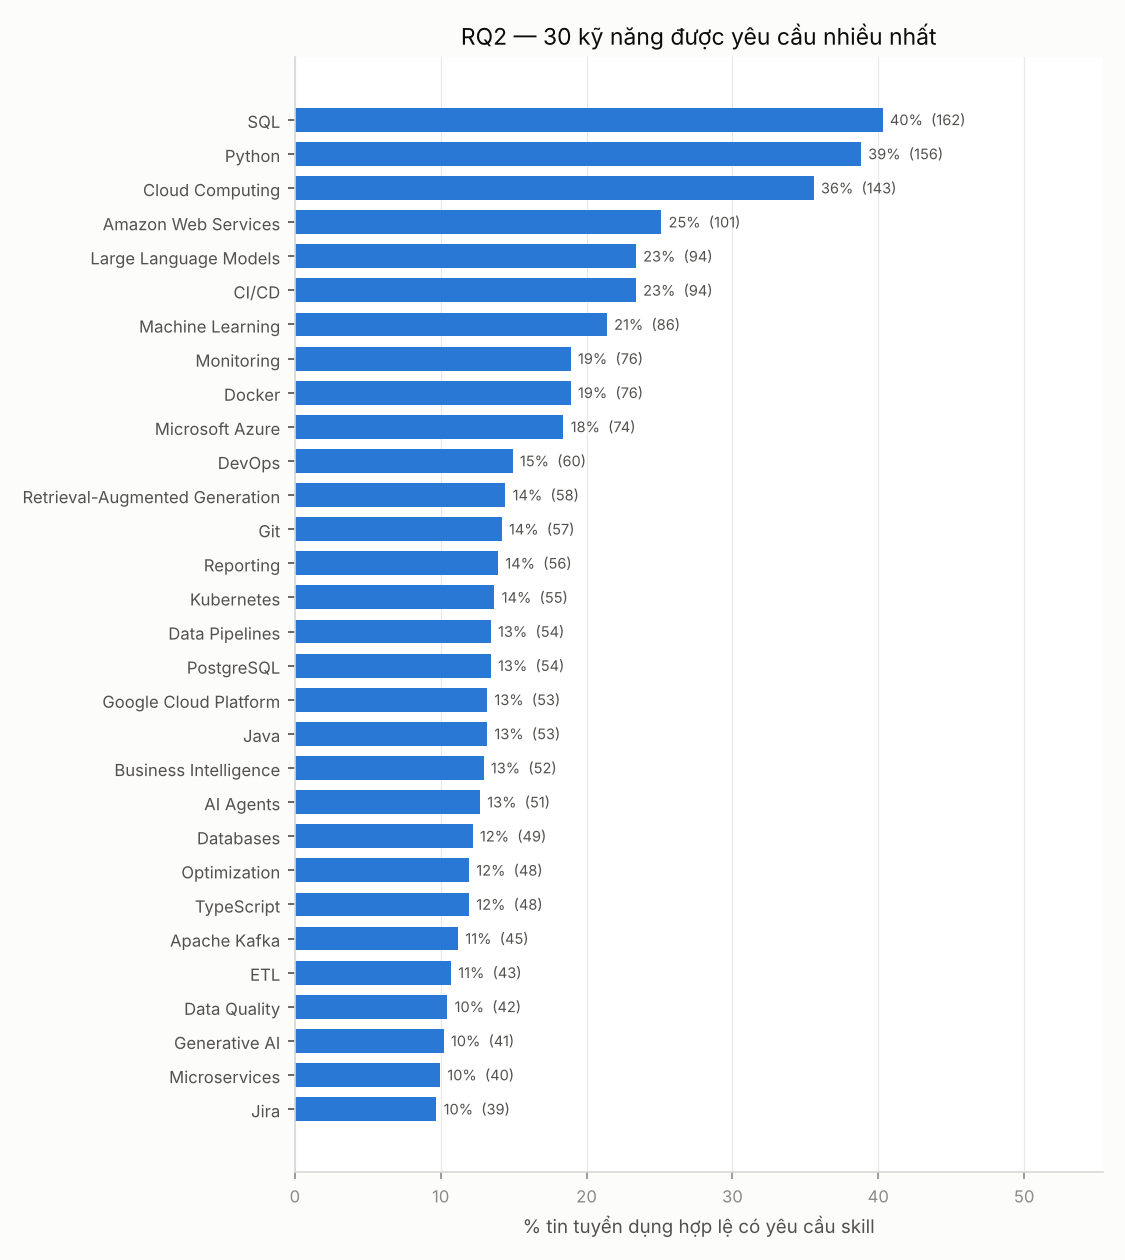
\includegraphics[width=0.85\textwidth]{image/rq2_top_skills.png}}{\fbox{rq2\_top\_skills.png}}
\caption{Các kỹ năng phổ biến nhất trong 402 tin hợp lệ}
\label{fig:topskills}
\end{figure}

SQL có trong 40\% số tin, Python 39\%, Cloud Computing 36\%, AWS 25\%, LLM 23\%, CI/CD 23\%, Machine Learning 21\%. SQL và Python ngang nhau trong khoảng sai số. Các cặp đi cùng nhau mạnh nhất (NPMI, cùng xuất hiện $\ge 5$ lần): PyTorch--TensorFlow 0,94; NumPy--Pandas 0,91; Grafana--Prometheus 0,89.

\subsection{RQ3: độ nhất quán của chức danh}

Chỉ 5 chức danh đạt ngưỡng 5 tin. Bảng~\ref{tab:rq3} so độ phân tán với phân vị 5\% của 1.000 lần bốc ngẫu nhiên cùng cỡ.

\begin{table}[htbp]
\centering
\caption{Độ phân tán của chức danh so với mốc ngẫu nhiên (sơ bộ)}
\label{tab:rq3}
\renewcommand{\arraystretch}{1.15}
\begin{tabular}{l r r r l}
\toprule
\textbf{Chức danh} & \textbf{Số tin} & \textbf{Phân tán} & \textbf{P5 ngẫu nhiên} & \textbf{Kết luận} \\
\midrule
Data Engineer & 13 & 0,77 & 0,91 & nhất quán \\
AI Engineer & 9 & 0,84 & 0,91 & nhất quán \\
IT Business Analyst & 6 & 0,85 & 0,89 & nhất quán \\
Data Analyst & 5 & 0,893 & 0,888 & không phân biệt được \\
Business Analyst & 11 & 0,96 & 0,91 & không phân biệt được \\
\bottomrule
\end{tabular}
\end{table}

Ví dụ cách tính cho Data Engineer: 13 tin tạo 78 cặp; cặp giống nhất chung 8 trên 18 kỹ năng (Jaccard 0,44), cặp ở mức giữa chung 11 trên 49 (0,22); Jaccard trung bình 0,23 nên phân tán 0,77. Trong 1.000 lần bốc 13 tin bất kỳ, lần giống nhau nhất cũng chỉ có phân tán 0,88. Kết quả của Business Analyst không có nghĩa tên ``BA'' vô nghĩa, mà là \textit{xét theo kỹ năng kỹ thuật} các tin BA không giống nhau, vì chúng chỉ có khoảng 3 kỹ năng kỹ thuật và mô tả công việc bằng nghiệp vụ, phần taxonomy không đo.

\subsection{RQ4: phân cụm}
\label{sec:res-rq4}

\textbf{Lần chạy theo đường ống (Euclid).} Luật chọn $k$ cho $k = 2$; silhouette 0,03; ARI giữa cụm và chức danh 0,002; ARI giữa K-Means và phân cụm phân cấp $-0{,}05$ (phân cụm phân cấp dồn 381 tin vào một cụm). Hai cụm K-Means khác nhau chủ yếu ở \textit{số lượng} kỹ năng: trung bình 21 và 6 kỹ năng mỗi tin. Thuật toán tách tin dài khỏi tin ngắn, không tách nghề (mục~\ref{sec:clustering}).

\textbf{Thử nghiệm khám phá với khoảng cách cosine} \dexuat{}. Silhouette của dữ liệu thật 0,09--0,11 so với 0,02--0,05 của dữ liệu xáo trộn, trên cả 402 tin lẫn 217 tin có chức danh Data/AI: có cấu trúc thật, dù yếu. Luật chọn $k$ trên 217 tin Data/AI vẫn chọn $k = 2$ (độ ổn định 0,89, so với 0,56--0,58 ở $k = 3$--$4$ và giảm dần đến 0,33). Hai cụm là nhánh \textbf{Dữ liệu} (98 tin: SQL 80\%, BI, chất lượng dữ liệu, ETL) và nhánh \textbf{AI} (118 tin: LLM 61\%, Machine Learning 52\%, RAG, CI/CD). Ở $k = 4$, bốn cụm nằm gọn trong hai nhánh: Data Analyst/BI (48), Data Engineer (47), ứng dụng LLM (60), ML truyền thống (51).

\begin{table}[htbp]
\centering
\caption{Chức danh $\times$ cụm ở $k = 4$ (khám phá, độ ổn định 0,58; nhóm chức danh bằng từ khoá thô)}
\label{tab:crosstab}
\renewcommand{\arraystretch}{1.15}
\small
\begin{tabular}{l r r r r r}
\toprule
\textbf{Chức danh} & \textbf{Kỹ nghệ DL} & \textbf{ML} & \textbf{Phân tích/BI} & \textbf{LLM} & \textbf{Tổng} \\
\midrule
AI Engineer / LLM & 7 & \textbf{29} & 6 & \textbf{54} & 96 \\
Data Engineer & \textbf{30} & 2 & 1 & 1 & 34 \\
Data Analyst & 2 & 0 & \textbf{13} & 0 & 15 \\
Data Scientist & 2 & \textbf{8} & 2 & 0 & 12 \\
ML Engineer & 1 & \textbf{12} & 0 & 0 & 13 \\
\bottomrule
\end{tabular}
\end{table}

Chức danh phổ biến nhất, ``AI Engineer'', gồm ít nhất hai việc khác nhau: khoảng 56\% là kỹ sư ứng dụng LLM, 30\% là việc huấn luyện mô hình kiểu ML Engineer. Data Engineer và Data Analyst khoảng 88\% nằm đúng cụm. Data Scientist ở Việt Nam nghiêng về ML (8/12 tin, quá ít để kết luận). Mức $k = 4$ kém ổn định nên chỉ được trình bày như lớp chi tiết, kèm độ ổn định.

\newpage
% =====================================================================
\section{Thảo luận}
% =====================================================================
\subsection{Bài toán phải có ý nghĩa với người dùng}

Phát biểu ban đầu đo ``mức lệch giữa tên và kỹ năng''. Đó là câu hỏi đúng về mặt nghiên cứu nhưng không trả lời được ``đo để làm gì''. Chỉ kết luận ``thị trường chia thành Dữ liệu và AI'' thì ai cũng biết, không cần nghiên cứu; phân cụm ra $k = 2$ thực chất là phép kiểm tra phương pháp chạy đúng. Giá trị nằm ở chỗ người thường không tự đoán được: chức danh nào đáng tin, chức danh nào là nhiều việc khác nhau, và một danh sách kỹ năng dài thì thực chất là việc gì. Vì vậy khung mới đặt người tìm việc vào trung tâm và biến câu hỏi phân loại thành một bài toán có đáp án do người gán, chấm được bằng macro-F1, so được nhiều phương pháp.

\subsection{Thị trường liên tục hơn là phân ô}

Silhouette quanh 0,1 nghĩa là các nhóm chồng lên nhau nhiều. Thị trường giống một dải liên tục có nhiều vai trò lai hơn là các ô tách bạch. Đây là một phát hiện, cần trình bày trung thực kèm mốc dữ liệu xáo trộn làm bằng chứng. Nó cũng là lý do thử mô hình hỗn hợp (LDA, NMF), cho phép một tin thuộc nhiều vai trò thay vì gán cứng vào một cụm.

\subsection{Bộ lọc liên quan và phạm vi Business Analyst}

Phạm vi ban đầu không nhắc BA ở đâu, nhưng crawler chủ động thu danh mục BA; bộ lọc ``một từ khoá là đủ'' và bước giữ mặc định làm 68 tin BA và 117 tin IT chung lọt vào. Lỗi không thuộc riêng ai: quy tắc mặc định ``giữ rồi rà soát tay'' là thiết kế có chủ đích nhưng chưa ai rà soát, và quy tắc chỉ được thử trên mẫu 45 tin. Khi bài toán chuyển sang giúp người mới đọc đúng tin, nhầm lẫn BA và Data Analyst lại chính là một nỗi đau thật, nên BA được giữ làm một lớp riêng thay vì loại hẳn.

\subsection{Vai trò của trợ lý AI trong quy trình}

Nhóm dùng trợ lý AI để viết mã, gán nhãn nháp kỹ năng (Codex), rà soát lượt hai (Claude) và soạn tài liệu. Để tránh ``máy chấm máy'': nhãn nháp được làm trước khi chạy bộ trích xuất; mọi nhãn phải được người duyệt; 18 tin kappa được gán khi nhãn nháp bị ẩn; quyết định quy ước (như API Design) do người đưa ra và ghi lại. Một bản duyệt giống y hệt nhãn nháp là dấu hiệu bấm đồng ý theo thói quen và cần được kiểm tra lại.

\newpage
% =====================================================================
\section{Hạn chế}
% =====================================================================

\textbf{Một nguồn, một khung thời gian.} Chỉ ITviec, thu từ 30/09 đến 23/11/2026. ITviec thiên về công ty công nghệ và tin tiếng Anh. Mọi kết luận chỉ nói về ``tin đăng trên ITviec trong khung này''; không phân tích xu hướng.

\textbf{Cỡ mẫu nhỏ.} Khoảng 400 tin hợp lệ, có thể khoảng 300 sau khi siết bộ lọc, sát ngưỡng phân cụm. Nhiều chức danh dưới 5 tin, nhiều cặp kỹ năng dưới 5 lần. Các ngưỡng loại bỏ phép đo không đủ dữ liệu và liệt kê phần bị loại.

\textbf{Tin tuyển dụng không phải công việc thực tế.} Tin thường liệt kê kỹ năng mong muốn quá rộng hoặc chép mẫu cũ. Kết quả trả lời ``nhà tuyển dụng \textit{viết} gì'', không phải ``người làm nghề \textit{làm} gì''.

\textbf{Crawler.} Chưa lấy được địa điểm ở 29\% tin và kinh nghiệm ở mọi tin. Pilot dùng parser v0.2 nên khoảng trắng gốc không còn. Trùng gần khác chức danh (cặp MB Bank \#36/\#40) chưa bị bắt vì luồng chỉ dựa vào mô tả đang tắt.

\textbf{Bộ trích xuất.} Dựa trên từ điển, không hiểu ngữ cảnh và phủ định; thiếu tên tiếng Việt và nhiều tên gọi khác; đọc cả phần giới thiệu công ty. Recall thấp làm danh sách kỹ năng ngắn hơn thực tế, làm phồng độ phân tán ở RQ3 và làm yếu liên kết ở RQ2; mốc ngẫu nhiên ở RQ3 chịu cùng mức thiếu nên phép so vẫn công bằng. Taxonomy khoá ngày 23/11 nên kỹ năng mới sau đó không được bắt.

\textbf{Bộ đáp án.} Gold là 50 tin ngắn nhất, có thể không đại diện cho tin dài; nhãn nháp do AI gán; chỉ 18 tin được hai người gán độc lập; holdout 23 tin nên khoảng tin cậy rộng.

\textbf{Chuẩn hoá chức danh và nhãn vai trò.} Chuẩn hoá theo luật nên hai chức danh thực chất giống nhau vẫn có thể tách riêng; RQ3, RQ4 nhạy với luật này. Bảy vai trò là một định nghĩa của nhóm, có ranh giới mờ (DS/MLE, MLE/AIE).

\textbf{Phương pháp.} Các ngưỡng là lựa chọn phương pháp luận, không phải giá trị chuẩn, nhưng được chốt trước khi xem dữ liệu thật. K-Means giả định cụm dạng cầu trên dữ liệu nhị phân thưa, nên có phân cụm phân cấp đối chứng. Nghiên cứu mang tính mô tả và khám phá, không khẳng định nhân quả.

\textbf{Điều khoản sử dụng.} Không công bố lại văn bản tin; báo cáo chỉ dùng số liệu tổng hợp và trích đoạn ngắn; dữ liệu thô không đưa lên kho mã công khai.

\newpage
% =====================================================================
\section{Tiến độ và kế hoạch}
\label{sec:progress}
% =====================================================================

\begin{table}[htbp]
\centering
\caption{Tiến độ đến ngày 08/11/2026}
\label{tab:progress}
\renewcommand{\arraystretch}{1.15}
\begin{tabularx}{\textwidth}{>{\raggedright\arraybackslash}p{4.6cm} X}
\toprule
\textbf{Hạng mục} & \textbf{Tình trạng} \\
\midrule
Phạm vi, lược đồ, quy tắc chất lượng & \textbf{Xong.} Lược đồ 22 trường khoá; quyết định ghi ở Phụ lục~\ref{app:decisions} \\
Thu thập & \textbf{Hai đợt xong} (504 tin). Còn sửa crawler (địa điểm, kinh nghiệm), thu 15/11 và 22/11 \\
Làm sạch, RQ1 & \textbf{Xong phiên bản 1.} Còn siết bộ lọc liên quan \\
Taxonomy, bộ trích xuất & \textbf{Xong phiên bản 1.} Còn bổ sung tên gọi (tiếng Việt, REST API) trước 23/11 \\
Gold kỹ năng & \textbf{Đang duyệt.} Nhãn nháp, góp ý lượt hai, công cụ duyệt và script gộp đã có; chưa có kappa \\
Đường ống, kiểm tra chất lượng & \textbf{Xong.} 302 kiểm thử đạt \\
EDA & \textbf{Xong} trên dữ liệu chưa chốt \\
RQ2--RQ4 & \textbf{Bản chạy thử.} Còn đổi K-Means sang cosine, thêm mốc xáo trộn, khoảng tin cậy \\
Nhãn vai trò & \textbf{Công cụ sẵn sàng.} Hướng dẫn, mẫu 300 tin, trang gán nhãn, script gộp; chưa gán \\
Nhiệm vụ 1--3, ứng dụng web, khảo sát & \textbf{Chưa làm} \\
\bottomrule
\end{tabularx}
\end{table}

\begin{table}[htbp]
\centering
\caption{Kế hoạch các giai đoạn còn lại}
\label{tab:plan}
\renewcommand{\arraystretch}{1.15}
\begin{tabularx}{\textwidth}{l X >{\raggedright\arraybackslash}p{3.6cm}}
\toprule
\textbf{Thời gian} & \textbf{Công việc} & \textbf{Kết quả} \\
\midrule
08--14/11 & Gán nhãn vai trò 300 tin (cả nhóm); duyệt gold kỹ năng và tính kappa; khảo sát sinh viên; sửa crawler; sao lưu dữ liệu thô & Nhãn vai trò, $\kappa$, bằng chứng nhu cầu \\
15--22/11 & Thu đợt 15/11 và 22/11; bổ sung tên gọi từ nửa tune; siết bộ lọc; mã Nhiệm vụ 1 và 2; đổi khoảng cách phân cụm & Bản thử Nhiệm vụ 1 \\
23/11 & \textbf{Chốt dữ liệu, taxonomy và bộ trích xuất}; ghi mã băm tệp dữ liệu & Bộ dữ liệu cuối \\
24/11--07/12 & Chấm bộ trích xuất trên holdout; chạy chính thức Nhiệm vụ 1--3 và RQ1--RQ4; ứng dụng web & Kết quả chính thức, ứng dụng \\
08--15/12 & Thử ứng dụng với 8--10 sinh viên; viết báo cáo cuối và slide & Báo cáo cuối kỳ \\
\bottomrule
\end{tabularx}
\end{table}

% =====================================================================
\section{Kết luận}
% =====================================================================
Đến nay nhóm đã có đủ chuỗi từ thu thập, làm sạch, trích xuất kỹ năng đến phân tích, chạy lại được bằng một lệnh và có kiểm tra chất lượng ở mỗi khâu, cùng 504 tin tự thu thập (402 tin hợp lệ). Kết quả sơ bộ cho thấy bộ trích xuất ít bắt nhầm nhưng bỏ sót khoảng một phần sáu kỹ năng, nhất là ở tin tiếng Việt; cách đặt tên chức danh phân mảnh thật; và chức danh phổ biến nhất, ``AI Engineer'', gồm ít nhất hai loại việc khác nhau. Phân tích khám phá cũng chỉ ra hai lỗi phương pháp mà nhóm tự phát hiện: bộ lọc liên quan quá lỏng, và K-Means với khoảng cách Euclid chia tin theo độ dài thay vì theo nghề.

Sau góp ý của giảng viên, bài toán được đặt lại quanh người tìm việc: nhận diện vai trò thật của một tin, tách kỹ năng cốt lõi, và đối chiếu kỹ năng của một người với các vai trò. Việc cần làm trước tiên là gán nhãn vai trò cho 300 tin và hoàn tất duyệt gold, vì mọi phép chấm phía sau đều dựa vào hai bộ đáp án này.

\chuaviet{Viết lại phần kết luận ở báo cáo cuối kỳ, sau khi có kết quả chính thức trên dữ liệu đã chốt.}

\newpage
\appendix
% =====================================================================
\section{Dữ liệu và mã nguồn}
\label{app:code}
% =====================================================================
Kho mã: \code{github.com/DuongXD-27/occupational-skill-structure-mining} (công khai), Python 3.11. Dữ liệu thô và dữ liệu đã xử lý (\code{data/raw/}, \code{data/processed/}, \code{data/features/}) bị \code{.gitignore} chặn và \textbf{không có trên GitHub}; chỉ mẫu nhỏ (\code{data/sample/}, \code{data/pilot/}) được theo dõi. Dữ liệu thô của các đợt thu phải được sao lưu ở thư mục chung của nhóm.

\textbf{Cấu trúc thư mục chính.}
\begin{itemize}[noitemsep, topsep=2pt, leftmargin=2.5em]
\item \code{src/crawler/}: crawler ITviec (\code{main.py}, \code{fetcher.py}, \code{listing.py}, \code{parser.py}) và TopCV (\code{topcv.py}).
\item \code{src/cleaner/}: QR-01 đến QR-06 (\code{pipeline.py}, \code{location.py}, \code{title.py}, \code{duplicates.py}, \code{relevance.py}) và RQ1 (\code{rq1.py}).
\item \code{src/parser/}: bộ trích xuất (\code{skill\_extractor.py}), xuất đặc trưng (\code{features.py}), đánh giá (\code{evaluation.py}).
\item \code{src/analysis/}: ngưỡng (\code{config.py}), kiểm tra chất lượng (\code{quality.py}), EDA (\code{eda.py}), RQ2--RQ4 (\code{rq2.py}, \code{rq3.py}, \code{rq4.py}), biểu đồ (\code{plots.py}), điều phối (\code{report.py}).
\item \code{src/pipeline/}: khung tích hợp, hợp đồng dữ liệu (\code{contracts.py}).
\item \code{taxonomy/skills\_taxonomy.csv}: taxonomy kỹ năng; \code{taxonomy/taxonomy\_gaps.csv}: công cụ gặp trong gold nhưng chưa có trong taxonomy.
\item \code{config/pipeline.json}, \code{config/pipeline\_itviec.json}: cấu hình đường ống; \code{config/location\_mapping.csv}: bảng ánh xạ địa điểm.
\item \code{reports/}: đầu ra sinh khi chạy (bảng, hình), không đưa lên GitHub.
\item \code{data/evaluation/}: gold nháp, góp ý lượt hai, \code{manifest.json}, \code{reviews/} (tệp duyệt).
\item \code{data/labels/}: mẫu gán nhãn vai trò, \code{role\_reviews/} (tệp gán nhãn), kết quả gộp.
\item \code{tools/gold\_review/}, \code{tools/role\_labeling/}: trang duyệt gold và trang gán nhãn vai trò chạy offline.
\item \code{notebooks/} (EDA, phân tích); \code{tests/} (kiểm thử); \code{report/} (báo cáo này).
\end{itemize}

\textbf{Lệnh thường dùng} (chạy từ thư mục gốc).
\begin{Verbatim}
# Cài đặt và kiểm thử
python -m pip install -r requirements.txt
python -m pytest -q

# Thu thập và gộp các đợt (giữ bản thu sớm nhất, khung 30/09-23/11 giờ VN)
python -m src.crawler.main --source itviec
python scripts/combine_raw.py data/pilot/jobs_pilot.jsonl data/raw/itviec/*.jsonl --output data/raw/jobs_raw.jsonl

# Toàn bộ đường ống: dữ liệu mẫu 45 tin / dữ liệu ITviec thật (đọc data/raw/jobs_raw.jsonl)
python -m src.pipeline --config config/pipeline.json --stage all
python -m src.pipeline --config config/pipeline_itviec.json --stage all

# Tải lại vài trang tin để tìm chỗ hiển thị địa điểm, kinh nghiệm (sửa crawler);
# HTML lưu ở data/raw/html_samples/, chỉ cần gửi lại report.json
python scripts/inspect_itviec_pages.py
python scripts/run_analysis.py --ignore-quality      # chỉ để chẩn đoán

# Taxonomy và bộ trích xuất
python scripts/recount_taxonomy.py --check
python -m src.parser preview --input data/sample/sample_jobs.jsonl --output-dir data/features/development
python -m src.parser extract --input data/processed/jobs_clean.parquet --output-dir data/features
python -m src.parser evaluate --gold data/evaluation/gold_jobs.reviewed.jsonl --output-dir reports/skill_extraction/tune --subset tune
python -m src.parser evaluate --gold data/evaluation/gold_jobs.reviewed.jsonl --output-dir reports/skill_extraction/holdout --subset holdout   # chỉ sau 23/11

# Duyệt gold kỹ năng
python tools/gold_review/build.py            # dựng tools/gold_review/index.html
python scripts/merge_gold_reviews.py          # gộp data/evaluation/reviews/*.json, tính kappa
python scripts/merge_gold_reviews.py --prefer cuong

# Gán nhãn vai trò
python scripts/sample_role_labeling.py --clean data/processed/jobs_clean.parquet
python tools/role_labeling/build.py --clean data/processed/jobs_clean.parquet   # index.html: không commit
python scripts/merge_role_labels.py

# EDA
python -m src.analysis.eda --raw data/raw/jobs_raw.jsonl --clean data/processed/jobs_clean.parquet --out reports/eda
\end{Verbatim}

\textbf{Cấu hình đường ống.} \code{config/pipeline.json} chạy trên 45 tin mẫu (\code{run\_kind = integration}); \code{config/pipeline\_itviec.json} giống hệt nhưng đọc \code{data/raw/jobs\_raw.jsonl} và chạy chế độ \code{research}. Mỗi tệp cấu hình có \code{version = 1}, \code{run\_kind} (\code{integration} khi thử, \code{research} khi chạy nghiên cứu với dữ liệu thật), \code{paths} (\code{raw}, \code{clean}, \code{skills}, \code{matrix}, \code{taxonomy}, \code{rq1}, \code{analysis}, \code{report}; tính từ thư mục của tệp cấu hình, không được trùng hay lồng nhau), \code{modules} (\code{module:function} của từng bước) và \code{options} (chuyển nguyên cho module). Chỉ dùng cấu hình tin cậy vì entry point được thực thi như mã Python.

\textbf{Trang duyệt gold.} Mở \code{tools/gold\_review/index.html} bằng trình duyệt, nhập tên, duyệt từng tin: giữ, sửa, bỏ nhãn; chọn thêm hay bỏ qua từng góp ý; thêm kỹ năng bị sót bằng cách bôi đoạn văn bản. Trang tự lưu trong trình duyệt; bấm ``Xuất'' để tải \code{gold\_review\_<tên>.json} rồi đặt vào \code{data/evaluation/reviews/}. Với 18 tin kappa, phải gán độc lập trước khi nhãn nháp hiện ra. Sửa trang ở \code{template.html} và \code{app.js}, sau đó chạy lại \code{build.py}.

\textbf{Trang gán nhãn vai trò.} Trưởng nhóm dựng \code{index.html} trên máy có dữ liệu và gửi cho thành viên qua thư mục chung. Mỗi người mở trang, nhập tên, chọn lô được giao, gán nhãn, bấm ``Xuất kết quả'' và đặt \code{role\_labels\_<tên>.json} vào \code{data/labels/role\_reviews/}.

% =====================================================================
\section{Nhật ký quyết định}
\label{app:decisions}
% =====================================================================
Trưởng nhóm (Dương) chốt mọi thay đổi về phạm vi, lược đồ và tiêu chuẩn giữ/loại tin; thành viên không đổi các quy ước này để hợp với mã riêng. Quyết định mới được thêm vào cuối bảng.

\begin{longtable}{>{\raggedright\arraybackslash}p{2.2cm} >{\raggedright\arraybackslash}p{12.4cm}}
\caption{Các quyết định của đồ án}\label{tab:decisions}\\
\toprule
\textbf{Ngày} & \textbf{Quyết định} \\
\midrule
\endfirsthead
\toprule
\textbf{Ngày} & \textbf{Quyết định} \\
\midrule
\endhead
09/2026 & Phạm vi, bốn câu hỏi nghiên cứu, ITviec là nguồn chính, TopCV dự phòng; tối đa hai nguồn; không vượt CAPTCHA hay chống bot. \\
15/09/2026 & Hướng dẫn gán nhãn kỹ năng (bản pilot); taxonomy 246 kỹ năng từ 45 tin mẫu. \\
24/09/2026 & Đặc tả phân tích: chỉ số và ngưỡng của RQ1--RQ4 viết trước khi có dữ liệu. \\
03/10/2026 & \textbf{A.} Phân công: Đạt thu thập; Đức làm sạch, chuẩn hoá chức danh và RQ1; Cường trích xuất kỹ năng; Triều RQ2--RQ4; Dương phạm vi, lược đồ, điều phối, nghiệm thu. \textbf{C.} \code{raw\_job\_title} giữ nguyên văn nguồn, crawler không ghép thêm công nghệ; ``Senior Data Analyst'', ``Data Analyst'', ``DATA ANALYST'' chuẩn hoá thành ``Data Analyst''; không mặc định gộp AI Engineer, ML Engineer, Data Scientist. \textbf{D.} Bảng sạch giữ mọi bản ghi; tập phân tích là \code{relevance\_flag = true AND duplicate\_flag = false}; \code{quality\_flags} ghi ở tệp riêng. Bỏ ba trường lương phái sinh (29 xuống 26 trường). \\
04/10/2026 & \textbf{B.} Bỏ \code{experience\_min\_years}, \code{experience\_max\_years}, \code{salary\_raw}, \code{education}; lược đồ còn 22 trường; chỉ giữ \code{raw\_experience} nguyên văn. Khung tích hợp đạt 49 kiểm thử. \\
11/10/2026 & Tích hợp bộ trích xuất; sửa lỗi khử trùng đoạn chồng; gold nháp 50 tin (634 nhãn, Codex gán). \\
03/11/2026 & \textbf{F.1} Kích hoạt TopCV (sau đó bị chặn HTTP 403, không dùng). \textbf{F.2} Bản sửa sau review đẩy vào nhánh thành viên, thứ tự merge \#15, \#12, \#13, \#14, \#16. \textbf{F.3} Gold do Cường và Dương duyệt; mỗi người gán độc lập 15--20 tin trước để đo kappa (chọn 18). \textbf{F.4} Cường duyệt gold, bổ sung tên gọi, số liệu P/R/F1. \textbf{F.5} Chuẩn hoá chức danh: chỉ bỏ cấp bậc thuần tuý; giữ Lead, Intern, Head; chỉ bỏ hậu tố khi mọi mục là công cụ trong taxonomy. \textbf{F.6} Luồng trùng gần chỉ dựa vào mô tả giữ tắt. \textbf{F.7} Khung quan sát 30/09--23/11; cùng URL giữ bản thu sớm nhất. \textbf{F.8} Pilot v0.2 được thu lại bằng v0.3 với tin còn đăng. \textbf{F.9} Khoá taxonomy và bộ trích xuất ngày 23/11; gold chia cố định tune/holdout. \textbf{F.10} Giữ nguyên các ngưỡng; RQ3 cần ít nhất 3 chức danh đạt 5 tin. \textbf{F.11} Luật chọn $k$: ổn định, rồi silhouette, rồi $k$ nhỏ (biên 0,02). \textbf{F.12} Không làm mô hình dự đoán chức danh cho RQ3. \textbf{F.13} Dưới 300 tin hợp lệ thì không hạ ngưỡng; RQ4 trình bày như phương pháp. Đề xuất tám bước kiểm tra chất lượng. \\
03/11/2026 & Chỉ dùng ITviec, thu nhiều đợt; gộp theo giờ Việt Nam. \\
05/11/2026 & Quy ước API Design (Cường): tin nhắc xây dựng, tích hợp hay làm việc với API đều gán API Design; không gán khi ``API'' là một phần tên sản phẩm. \\
07/11/2026 & Sau góp ý của giảng viên: đặt lại bài toán quanh người tìm việc với ba nhiệm vụ (mục~\ref{sec:problem}); bảy vai trò và hướng dẫn gán nhãn vai trò; giữ BA làm một lớp riêng, BA làm dữ liệu thuộc DA; MLOps gộp vào MLE; mẫu 300 tin gồm toàn bộ tin bị bộ lọc loại. \\
08/11/2026 & Gộp mọi tài liệu README và Markdown rải rác (trừ README ở thư mục gốc) vào báo cáo duy nhất \code{report/main.tex}. \\
\bottomrule
\end{longtable}

\textbf{Đang chờ duyệt:} tám bước kiểm tra chất lượng và ba ngưỡng cosine 0,70/0,80/0,90 của RQ3 (trưởng nhóm); giao thức đánh giá và tiêu chí chấp nhận ở mục~\ref{sec:protocol} (giảng viên); đổi K-Means sang cosine và thêm mốc dữ liệu xáo trộn.

% =====================================================================
\section{Hướng dẫn gán nhãn kỹ năng}
\label{app:skill-guideline}
% =====================================================================
Mục đích: các trường hợp cùng loại được xử lý giống nhau; người khác đọc hướng dẫn ra được quyết định tương tự; mỗi nhãn dựa trên một quy tắc rõ; không áp đặt danh mục nghề định sẵn. Định nghĩa kỹ năng và phạm vi ở mục~\ref{sec:taxonomy}.

\textbf{C.1 Vùng văn bản.} Lấy: phần yêu cầu, trách nhiệm, ``nice to have'', thẻ kỹ năng của vị trí, và chức danh \textit{chỉ khi} chức danh chứa rõ công nghệ (``Data Engineer (Python, Kafka)''). Không lấy: giới thiệu công ty, đãi ngộ, văn hoá công ty, việc làm tương tự, phần điều hướng, chính nhãn nghề. Công nghệ vừa ở phần giới thiệu vừa ở phần yêu cầu thì gán theo phần yêu cầu.

\textbf{C.2 Bắt buộc và ưu tiên.} Hiện tính cả hai, vì mục tiêu là bao phủ từ vựng. Giai đoạn sau có thể lưu thêm \code{requirement\_level} (\code{required}, \code{preferred}, \code{responsibility}).

\textbf{C.3 Viết tắt.} Viết tắt chuẩn, không mơ hồ thì ánh xạ thẳng: ML, DL, NLP, LLM(s), RAG, MCP, AWS, GCP, OCR, MLOps. ETL và ELT là hai kỹ năng khác nhau. Viết tắt mơ hồ chỉ ánh xạ khi đủ ngữ cảnh: ``CV'' chỉ là Computer Vision khi đi với OpenCV, ảnh hay video, nhận diện vật thể. Không suy ra khái niệm không được nhắc (có LLM không suy ra RAG).

\textbf{C.4 Đồng nghĩa và chính tả.} Biến thể chữ hoa, dấu cách, gạch nối, tên thông dụng về cùng tên chuẩn: Postgres $\rightarrow$ PostgreSQL; PowerBI $\rightarrow$ Power BI; sklearn $\rightarrow$ scikit-learn; MSSQL $\rightarrow$ Microsoft SQL Server; K8s $\rightarrow$ Kubernetes; GenAI $\rightarrow$ Generative AI. Không gộp hai công nghệ khác nhau dù hay đi cùng: PyTorch $\ne$ TensorFlow, AWS $\ne$ Azure, Data Lake $\ne$ Data Warehouse, RAG $\ne$ Vector Database.

\textbf{C.5 Cha--con.} Không suy kỹ năng cha từ con hay ngược lại: chỉ có ``SageMaker'' thì gán Amazon SageMaker, không thêm AWS; ``AWS SageMaker'' thì gán cả hai; Kubernetes không suy ra Docker; LangChain không suy ra RAG; LLM không suy ra Prompt Engineering. Dự án đo đúng điều nhà tuyển dụng viết.

\textbf{C.6 Kỹ năng ngầm.} Tuyệt đối không gán: ``xây dựng dashboard'' gán Dashboarding, không suy ra Power BI; ``deploy models'' gán Model Deployment, không suy ra Docker; ``làm việc với cơ sở dữ liệu quan hệ'' gán Relational Databases, không suy ra PostgreSQL.

\textbf{C.7 Liệt kê và lựa chọn.} Gán riêng từng công nghệ, kể cả khi tin nói ``một trong các'': C/C++ $\rightarrow$ C và C++; PyTorch/TensorFlow $\rightarrow$ hai kỹ năng; AWS/GCP/Azure $\rightarrow$ ba kỹ năng.

\textbf{C.8 Phụ thuộc ngữ cảnh.} Bài toán ứng dụng (fraud detection, credit scoring, customer analytics, cohort analysis, dynamic pricing) chỉ giữ khi vị trí phải xây dựng hoặc phân tích chúng, không giữ khi chỉ mô tả lĩnh vực kinh doanh. Quản trị, chất lượng, kiểm định, bảo mật, dòng dữ liệu giữ khi vị trí phải triển khai chúng; thuật ngữ pháp lý chung chung thì không. ``cloud'' chỉ thành Cloud Computing khi tin đòi hỏi kiến thức đám mây, không lấy ``công ty cloud'' ở phần giới thiệu. API Design, Microservices, CI/CD, Observability, Debugging được giữ.

\textbf{C.9 Quy ước API Design (05/11/2026).} Tin nhắc tới xây dựng, tích hợp hoặc làm việc với API (``build RESTful APIs'', ``REST/SOAP APIs'', ``API integrations'', ``tích hợp API'', ``familiarity with REST APIs'') đều gán API Design, kể cả khi chỉ nói dùng hay gọi API. Bằng chứng là cụm đầu tiên nhắc tới API. Không gán khi ``API'' là một phần tên sản phẩm (OpenAI API, FastAPI): gán kỹ năng tương ứng.

\textbf{C.10 Đếm.} Với mỗi tin: ánh xạ về tên chuẩn; khử trùng trong tin; mỗi kỹ năng nhận 0 hoặc 1. Thuật ngữ ngắn nằm trong thuật ngữ dài thì thuật ngữ dài thắng (``BI'' trong ``Power BI'' không tính Business Intelligence). Cẩn thận với CV (hồ sơ), R (trong R\&D), Go (từ thông thường).

\textbf{C.11 Mười lăm nhóm kỹ năng} (chỉ để quản lý từ vựng, không dùng làm nhãn nghề): Programming \& Query Languages; Data Analysis \& BI; Data Engineering \& Architecture; Distributed, Streaming \& Big Data; Databases, Storage \& Data Formats; Cloud Platforms \& Services; DevOps, MLOps \& Infrastructure; Machine Learning, Statistics \& Optimization; Generative AI \& Agentic Systems; NLP, Vision \& Multimodal AI; Software Engineering \& APIs; Data Quality, Testing \& Observability; Security Engineering; Applied Analytics \& Business Platforms; Engineering Tools \& Collaboration.

\textbf{C.12 Quy trình.} Đọc tin, đánh dấu đoạn kỹ thuật; áp dụng quy tắc lấy/loại; khái niệm đã có thì ánh xạ về tên chuẩn; khái niệm mới hợp lệ thì đề xuất kỹ năng mới qua quy trình quản lý taxonomy; biến thể của kỹ năng đã có thì đề xuất tên gọi khác; không gán kỹ năng ngầm; phân vân thì gắn cờ để hội ý, không đoán. Không xoá kỹ năng hiếm chỉ vì hiếm; trước hết kiểm tra nó là kỹ năng thật, tên gọi chưa gộp hay nhiễu.

\textbf{C.13 Cần xem lại sau.} Định dạng dữ liệu (CSV, XML, JSON) có nên là kỹ năng riêng; có nên có quan hệ cha--con chính thức (\code{parent\_skill\_id}); có nên lưu \code{requirement\_level} và \code{evidence\_span}; các bài toán ứng dụng tần suất thấp có nên giữ.

\textbf{C.14 So sánh với LLM (tuỳ chọn).} Bộ trích xuất theo luật và LLM phải được chấm trên cùng tập niêm phong, cùng hướng dẫn và cùng taxonomy; kết quả của LLM phải được ánh xạ về taxonomy trước khi tính P/R/F1, không cộng điểm cho khái niệm ngoài phạm vi.

% =====================================================================
\section{Hướng dẫn gán nhãn vai trò (v1, 07/11/2026)}
\label{app:role-guideline}
% =====================================================================
\textbf{D.1 Nguyên tắc vàng.} (1) Gán theo việc làm hằng ngày, không theo tên; công cụ ẩn chức danh và tên công ty; không tra tin trên mạng. (2) Câu hỏi quyết định: \textit{đầu ra chính của người này là gì?} (3) Đọc phần trách nhiệm trước, phần yêu cầu kỹ năng chỉ dùng để phân xử. (4) Cấp bậc không phải vai trò: Intern, Senior, Lead, Head vẫn gán theo lĩnh vực họ làm hay dẫn dắt. (5) Không chắc thì vẫn chọn, bật ``phân vân'' và ghi một dòng lý do.

\begin{longtable}{>{\raggedright\arraybackslash}p{1.4cm} >{\raggedright\arraybackslash}p{3.4cm} >{\raggedright\arraybackslash}p{4.4cm} >{\raggedright\arraybackslash}p{5.2cm}}
\caption{Bảy vai trò}\label{tab:roles}\\
\toprule
\textbf{Mã} & \textbf{Vai trò} & \textbf{Đầu ra chính} & \textbf{Dấu hiệu trong phần trách nhiệm} \\
\midrule
\endfirsthead
\toprule
\textbf{Mã} & \textbf{Vai trò} & \textbf{Đầu ra chính} & \textbf{Dấu hiệu trong phần trách nhiệm} \\
\midrule
\endhead
\code{DA} & Phân tích dữ liệu và BI & Báo cáo, dashboard, phân tích trả lời câu hỏi kinh doanh & xây báo cáo/dashboard, phân tích số liệu kinh doanh, theo dõi KPI, đưa ra insight \\
\code{DE} & Kỹ nghệ và quản trị dữ liệu & Pipeline, kho/hồ dữ liệu, mô hình dữ liệu, quy chuẩn dữ liệu & ETL/ELT, data warehouse/lakehouse, Spark/Airflow/Kafka, data governance, chất lượng dữ liệu, master data \\
\code{DS} & Khoa học dữ liệu & Mô hình thống kê/dự đoán \textit{để ra quyết định}, thí nghiệm & mô hình dự đoán churn/doanh số, A/B testing, phân tích thống kê, trình bày kết quả cho nghiệp vụ \\
\code{MLE} & Kỹ sư học máy (gồm MLOps, nghiên cứu mô hình) & Mô hình ML/DL \textit{được huấn luyện, tối ưu, triển khai} & train/fine-tune, thị giác máy tính, NLP, speech, tối ưu inference, model serving, MLOps, GPU \\
\code{AIE} & Kỹ sư ứng dụng AI (LLM) & Tính năng, sản phẩm \textit{dùng mô hình có sẵn} & tích hợp LLM/OpenAI API, RAG, AI agent, prompt engineering, vector database, chatbot \\
\code{BA} & Phân tích nghiệp vụ & Tài liệu yêu cầu, quy trình, user story & thu thập yêu cầu, viết BRD/SRS/user story, BPMN, cầu nối khách hàng và đội phát triển, UAT \\
\code{OTHER} & Không phải Data/AI & Phần mềm, hạ tầng, quản lý, kinh doanh & việc Data/AI dưới khoảng 1/3 khối lượng công việc \\
\bottomrule
\end{longtable}

\textbf{D.2 Quy ước.} BA mà việc chính là SQL, dashboard, phân tích số liệu: \code{DA}. BI developer, reporting analyst: \code{DA}. Analytics engineer (mô hình hoá dữ liệu bằng dbt cho BI): \code{DE}. Data governance, data quality, master data, data steward: \code{DE}. DBA vận hành cơ sở dữ liệu: \code{OTHER}. Product owner, project manager, kể cả ``AI Product Owner'': \code{OTHER} (có thể ghi vai trò phụ). Tư vấn, presales AI: \code{OTHER}. QA/tester, kể cả kiểm thử sản phẩm AI: \code{OTHER}, trừ khi việc chính là kiểm định mô hình hay dữ liệu. Backend ``biết dùng AI là lợi thế'': \code{OTHER}; backend mà phần lớn việc là LLM, RAG, agent: \code{AIE}. Kỹ sư thị giác, NLP, speech huấn luyện mô hình: \code{MLE}. Nghiên cứu viên AI: \code{MLE}. Head of Data, Data Manager: theo lĩnh vực họ dẫn dắt; trộn đều thì chọn mảng được mô tả nhiều nhất.

\textbf{D.3 Các cặp dễ nhầm.}
\begin{itemize}[noitemsep, topsep=2pt, leftmargin=2.5em]
\item \code{DA} hay \code{DS}: có xây mô hình dự đoán không? Chỉ mô tả, tổng hợp, trực quan hoá thì \code{DA}; hồi quy, phân loại, dự báo, A/B bài bản thì \code{DS}. ``Biết thống kê là lợi thế'' chưa đủ.
\item \code{DS} hay \code{MLE}: mô hình để ra quyết định hay chạy trong sản phẩm? Để phân tích, trình bày thì \code{DS}; đóng gói, triển khai, tối ưu tốc độ, phục vụ người dùng thì \code{MLE}.
\item \code{MLE} hay \code{AIE}: có huấn luyện hay tinh chỉnh mô hình không? Có thì \code{MLE}; chủ yếu gọi API mô hình có sẵn, ghép RAG, agent thì \code{AIE}. Fine-tune nhẹ (LoRA) chỉ là một ý trong tin chủ yếu về RAG/agent thì vẫn \code{AIE}.
\item \code{DE} hay \code{MLE}: pipeline phục vụ báo cáo, kho dữ liệu thì \code{DE}; phục vụ huấn luyện và triển khai mô hình (feature store, training pipeline, serving) thì \code{MLE}.
\item \code{DA} hay \code{BA}: đầu ra là số liệu hay tài liệu yêu cầu? SQL chỉ để ``tra cứu khi cần'' vẫn là \code{BA}.
\item \code{AIE}/\code{MLE}/\code{DE} hay \code{OTHER}: việc Data/AI dưới khoảng 1/3 phần trách nhiệm thì \code{OTHER}.
\end{itemize}

\textbf{D.4 Vai trò phụ và phân vân.} Chọn vai trò phụ chỉ khi tin thực sự lai, vai trò thứ hai chiếm khoảng 1/3 công việc trở lên (``xây pipeline \textit{và} dashboard cho ban giám đốc'': chính \code{DE}, phụ \code{DA}); không chọn chỉ vì tin liệt kê thêm vài kỹ năng. Bật ``phân vân'' khi hai vai trò gần ngang nhau hoặc tin quá ngắn, mơ hồ.

\begin{longtable}{>{\raggedright\arraybackslash}p{7.6cm} >{\raggedright\arraybackslash}p{1.3cm} >{\raggedright\arraybackslash}p{1.2cm} >{\raggedright\arraybackslash}p{4.3cm}}
\caption{Ví dụ gán nhãn vai trò (viết lại cho ngắn, không phải tin thật)}\label{tab:role-examples}\\
\toprule
\textbf{Đoạn trách nhiệm} & \textbf{Chính} & \textbf{Phụ} & \textbf{Lý do} \\
\midrule
\endfirsthead
\toprule
\textbf{Đoạn trách nhiệm} & \textbf{Chính} & \textbf{Phụ} & \textbf{Lý do} \\
\midrule
\endhead
Dashboard Power BI theo dõi doanh số; viết SQL; phân tích nguyên nhân sụt giảm & \code{DA} & -- & Báo cáo và phân tích \\
Pipeline Airflow nạp vào BigQuery; tối ưu job Spark; đảm bảo chất lượng dữ liệu & \code{DE} & -- & Pipeline, kho dữ liệu \\
Mô hình dự đoán khách hàng rời bỏ; thiết kế A/B test; trình bày cho marketing & \code{DS} & -- & Dự đoán để ra quyết định \\
Huấn luyện mô hình nhận diện biển số; tối ưu inference trên edge; triển khai bằng Triton & \code{MLE} & -- & Huấn luyện và triển khai \\
Chatbot nội bộ dùng GPT-4 và RAG; thiết kế prompt; vector DB; API FastAPI & \code{AIE} & -- & Dùng mô hình có sẵn \\
Hệ thống gợi ý: feature pipeline, huấn luyện mô hình xếp hạng, triển khai A/B & \code{MLE} & \code{DS} & Mô hình chạy trong sản phẩm \\
Thu thập yêu cầu khách hàng ngân hàng, viết user story, phối hợp đội dev, UAT & \code{BA} & -- & Tài liệu yêu cầu \\
Thu thập yêu cầu báo cáo, viết SQL, dựng dashboard Tableau cho các phòng ban & \code{DA} & \code{BA} & Đầu ra chính vẫn là số liệu \\
Backend Java Spring; tối ưu microservice; ưu tiên ứng viên từng dùng ChatGPT & \code{OTHER} & -- & Việc AI gần như không có \\
Quản lý sản phẩm AI: lộ trình, ưu tiên tính năng, phối hợp đội ML & \code{OTHER} & \code{AIE} & Vai trò quản lý \\
\bottomrule
\end{longtable}

\textbf{D.5 Cách làm việc và phân công đề xuất.} Lô K (60 tin) do Dương \textbf{và} Cường gán độc lập; B1 Dương, B2 Cường, B3 Đức, B4 Đạt, B5 Triều (mỗi lô 48 tin). Không trao đổi về các tin lô K cho đến khi cả hai đã xuất tệp. Sau khi gộp, nhóm họp thống nhất các tin bất đồng; bất đồng lặp lại theo một kiểu (ví dụ \code{DS}/\code{MLE}) thì sửa mục D.3, ghi ngày, và rà lại các tin cùng kiểu. Tiêu chí $\kappa \ge 0{,}6$ trên lô K; thấp hơn thì sửa hướng dẫn và gán lại lô K. Không sửa nhãn của mình sau khi đã thấy nhãn người khác ở lô K (chỉ sửa ở bước thống nhất, có lý do).

% =====================================================================
\section{Quy tắc chất lượng dữ liệu: chi tiết}
\label{app:quality}
% =====================================================================
\textbf{E.1 Xử lý giá trị thiếu (QR-01).}

{\small
\begin{longtable}{>{\raggedright\arraybackslash}p{4.2cm} >{\raggedright\arraybackslash}p{5cm} >{\raggedright\arraybackslash}p{5.2cm}}
\caption{Hành động khi thiếu trường}\label{tab:missing}\\
\toprule
\textbf{Trường thiếu} & \textbf{Hành động} & \textbf{Cờ} \\
\midrule
\endfirsthead
\toprule
\textbf{Trường thiếu} & \textbf{Hành động} & \textbf{Cờ} \\
\midrule
\endhead
\code{raw\_job\_title} & Loại bản ghi & \code{MISSING\_JOB\_TITLE} \\
\code{source}, \code{source\_url} & Loại bản ghi (không truy vết, không khử trùng được) & \code{MISSING\_SOURCE}, \code{MISSING\_SOURCE\_URL} \\
\code{source\_url} sai cú pháp & Loại bản ghi & \code{INVALID\_URL} \\
Cả mô tả và yêu cầu & Giữ; \code{relevance\_flag = false}, \code{INSUFFICIENT\_TEXT} & \code{MISSING\_TEXT\_FIELDS} \\
Cả hai có nhưng đều $<$ 30 ký tự; chức danh là trang lỗi & Giữ; \code{relevance\_flag = false}, \code{SCRAPE\_ERROR} & \code{SCRAPE\_FAILED}, \code{SCRAPE\_ERROR\_CONTENT} \\
Chỉ mô tả hoặc chỉ yêu cầu & Giữ; dùng trường còn lại & \code{MISSING\_JOB\_DESCRIPTION}, \code{MISSING\_JOB\_REQUIREMENTS} \\
Thời điểm thu, công ty, parser & Giữ; không điền giá trị giả & \code{MISSING\_*} \\
Địa điểm & Giữ; \code{normalized\_location = null} & \code{MISSING\_LOCATION} \\
Kinh nghiệm & Giữ; \code{null}, không suy diễn & \code{MISSING\_EXPERIENCE} \\
\bottomrule
\end{longtable}
}

\textbf{E.2 Ánh xạ địa điểm (QR-02)}, áp dụng sau khi cắt khoảng trắng, không phân biệt chữ hoa. Chuỗi chứa cả Hà Nội và TP. Hồ Chí Minh thì thành ``Nhiều địa điểm''.

\begin{longtable}{>{\raggedright\arraybackslash}p{9.6cm} >{\raggedright\arraybackslash}p{5cm}}
\caption{Bảng ánh xạ địa điểm (đầy đủ ở \code{location\_mapping.csv})}\label{tab:location}\\
\toprule
\textbf{Mẫu trên \code{raw\_location}} & \textbf{\code{normalized\_location}} \\
\midrule
\endfirsthead
\toprule
\textbf{Mẫu trên \code{raw\_location}} & \textbf{\code{normalized\_location}} \\
\midrule
\endhead
ha noi, hà nội, HN; quận Cầu Giấy, Thanh Xuân, Đống Đa, Ba Đình, \dots & Hà Nội \\
ho chi minh, hồ chí minh, HCM, HCMC, TP.HCM, sài gòn; Quận 1, Quận 7, Tân Bình, Thủ Đức, \dots & Hồ Chí Minh \\
da nang, đà nẵng; cần thơ; hải phòng; bình dương; đồng nai & Tên tỉnh/thành tương ứng \\
remote, WFH, work from home, làm việc từ xa, online & Remote \\
toàn quốc, nationwide, cả nước & Toàn quốc \\
Nhiều tỉnh/thành (dấu phẩy hoặc \code{/}) & Nhiều địa điểm \\
not available, n/a, unknown & \code{null} + \code{MISSING\_LOCATION} \\
Không khớp mẫu nào & \code{null} + \code{LOCATION\_UNRECOGNIZED} \\
\bottomrule
\end{longtable}

\textbf{E.3 Danh sách từ khoá Data/AI (QR-06, bước 2).} python, r language, sql, spark, hadoop, kafka, airflow, dbt, pandas, numpy, scikit-learn, tensorflow, pytorch, keras, machine learning, deep learning, neural network, nlp, llm, gpt, computer vision, data pipeline, etl, elt, data warehouse, data lake, power bi, tableau, looker, metabase, superset, data analyst, data engineer, data scientist, data architect, bi analyst, analytics engineer, mlops, llmops, vector database, embedding, rag, fine-tuning, statistics, regression, classification, clustering, recommendation system.

\textbf{E.4 Mẫu chức danh bị loại (QR-06, bước 1).} IT thuần: software engineer, web/mobile developer, devops engineer, system admin, network engineer, qa engineer, tester, sap specialist/mm/fico. Bán hàng, marketing: sales, marketing, business development, account manager, hr, recruiter, monetization specialist. Nhập liệu: data entry, data input, nhập liệu. Vận hành, tài chính: accountant, finance, logistics, supply chain, operations. Thiết kế: ui/ux designer, graphic designer. Quản lý chung: general manager, project manager, scholarship. Chức danh vừa có từ Data/AI vừa có từ bị loại (``AI Sales Manager''): mẫu loại thắng, thêm cờ \code{AMBIGUOUS\_CLASSIFICATION}.

\textbf{E.5 Nhãn \code{exclusion\_reason}.} \code{NOT\_DATA\_AI\_ROLE} (chức danh ngoài phạm vi), \code{DATA\_ENTRY\_ROLE} (nhập liệu thuần tuý), \code{INSUFFICIENT\_TEXT} (thiếu cả hai trường văn bản), \code{SCRAPE\_ERROR} (trang lỗi, nội dung hỏng). \code{MANUAL\_REVIEW\_REQUIRED} chỉ là cờ chất lượng: tin không khớp danh sách nào, vẫn được giữ.

\textbf{E.6 Cờ chất lượng khác.} \code{SENIORITY\_REMOVED}, \code{TECH\_SUFFIX\_REMOVED}, \code{RECRUITMENT\_NOISE\_REMOVED} (đã bỏ phần tương ứng khỏi chức danh chuẩn hoá); \code{AMBIGUOUS\_TITLE} (chức danh chứa hai vai trò); \code{TITLE\_TOO\_SHORT} ($<$ 3 ký tự), \code{TITLE\_TOO\_LONG} ($>$ 100 ký tự); \code{DESCRIPTION\_TOO\_SHORT} (mô tả $<$ 50 ký tự); \code{DUPLICATE\_EXACT}, \code{DUPLICATE\_NEAR}, \code{SENIORITY\_VARIANT}; \code{MULTI\_LOCATION}; \code{SCRAPER\_FIELD\_MISMATCH} (crawler gán nhầm hình thức làm việc vào kinh nghiệm).

\textbf{E.7 Ngưỡng cảnh báo.} Trên 10\% tin thiếu cả hai trường văn bản: dừng. Trên 20\% thiếu yêu cầu, trên 30\% thiếu địa điểm, trên 15\% tin bị đánh dấu trùng: ghi cảnh báo và kiểm tra crawler.

% =====================================================================
%  TÀI LIỆU THAM KHẢO
% =====================================================================
\clearpage
\phantomsection
\addcontentsline{toc}{section}{Tài liệu tham khảo}

\begin{thebibliography}{99}

\bibitem{blei2003lda}
D.~M.~Blei, A.~Y.~Ng and M.~I.~Jordan.
\newblock ``Latent Dirichlet Allocation.''
\newblock \emph{Journal of Machine Learning Research}, 3:993--1022, 2003.

\bibitem{blondel2008louvain}
V.~D.~Blondel, J.-L.~Guillaume, R.~Lambiotte and E.~Lefebvre.
\newblock ``Fast unfolding of communities in large networks.''
\newblock \emph{Journal of Statistical Mechanics: Theory and Experiment}, P10008, 2008.

\bibitem{bouma2009npmi}
G.~Bouma.
\newblock ``Normalized (Pointwise) Mutual Information in Collocation Extraction.''
\newblock \emph{Proceedings of GSCL}, 2009.

\bibitem{cohen1960kappa}
J.~Cohen.
\newblock ``A Coefficient of Agreement for Nominal Scales.''
\newblock \emph{Educational and Psychological Measurement}, 20(1):37--46, 1960.

\bibitem{davies1979db}
D.~L.~Davies and D.~W.~Bouldin.
\newblock ``A Cluster Separation Measure.''
\newblock \emph{IEEE Transactions on Pattern Analysis and Machine Intelligence}, 1(2):224--227, 1979.

\bibitem{efron1979bootstrap}
B.~Efron.
\newblock ``Bootstrap Methods: Another Look at the Jackknife.''
\newblock \emph{The Annals of Statistics}, 7(1):1--26, 1979.

\bibitem{hubert1985ari}
L.~Hubert and P.~Arabie.
\newblock ``Comparing Partitions.''
\newblock \emph{Journal of Classification}, 2(1):193--218, 1985.

\bibitem{landis1977kappa}
J.~R.~Landis and G.~G.~Koch.
\newblock ``The Measurement of Observer Agreement for Categorical Data.''
\newblock \emph{Biometrics}, 33(1):159--174, 1977.

\bibitem{lange2004stability}
T.~Lange, V.~Roth, M.~L.~Braun and J.~M.~Buhmann.
\newblock ``Stability-Based Validation of Clustering Solutions.''
\newblock \emph{Neural Computation}, 16(6):1299--1323, 2004.

\bibitem{rousseeuw1987silhouette}
P.~J.~Rousseeuw.
\newblock ``Silhouettes: A Graphical Aid to the Interpretation and Validation of Cluster Analysis.''
\newblock \emph{Journal of Computational and Applied Mathematics}, 20:53--65, 1987.

\end{thebibliography}

\end{document}
